\chapter{Analysis}
\label{appendix-analysis}

\section{Modular analysis}
\label{appendix-modular-analysis}

\begin{figure}[H]
\begin{subfigure}{0.45\textwidth}
	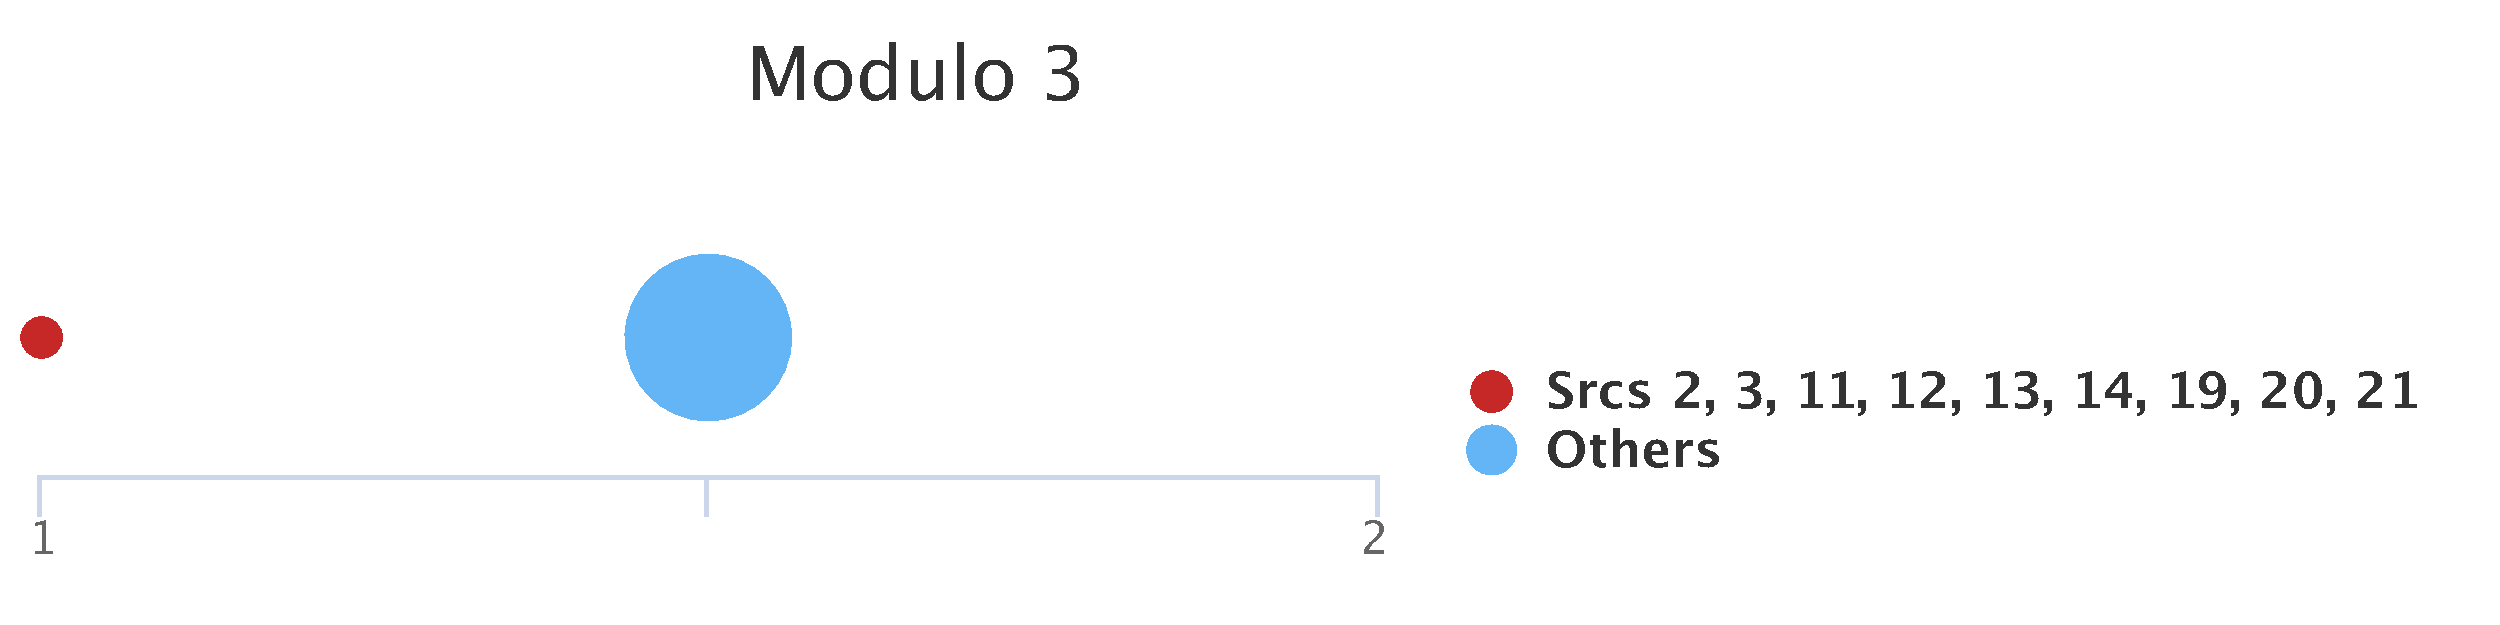
\includegraphics[width=\linewidth]{tex/images/analysis/mod3}
\end{subfigure}
\hfill
\begin{subfigure}{0.45\textwidth}
	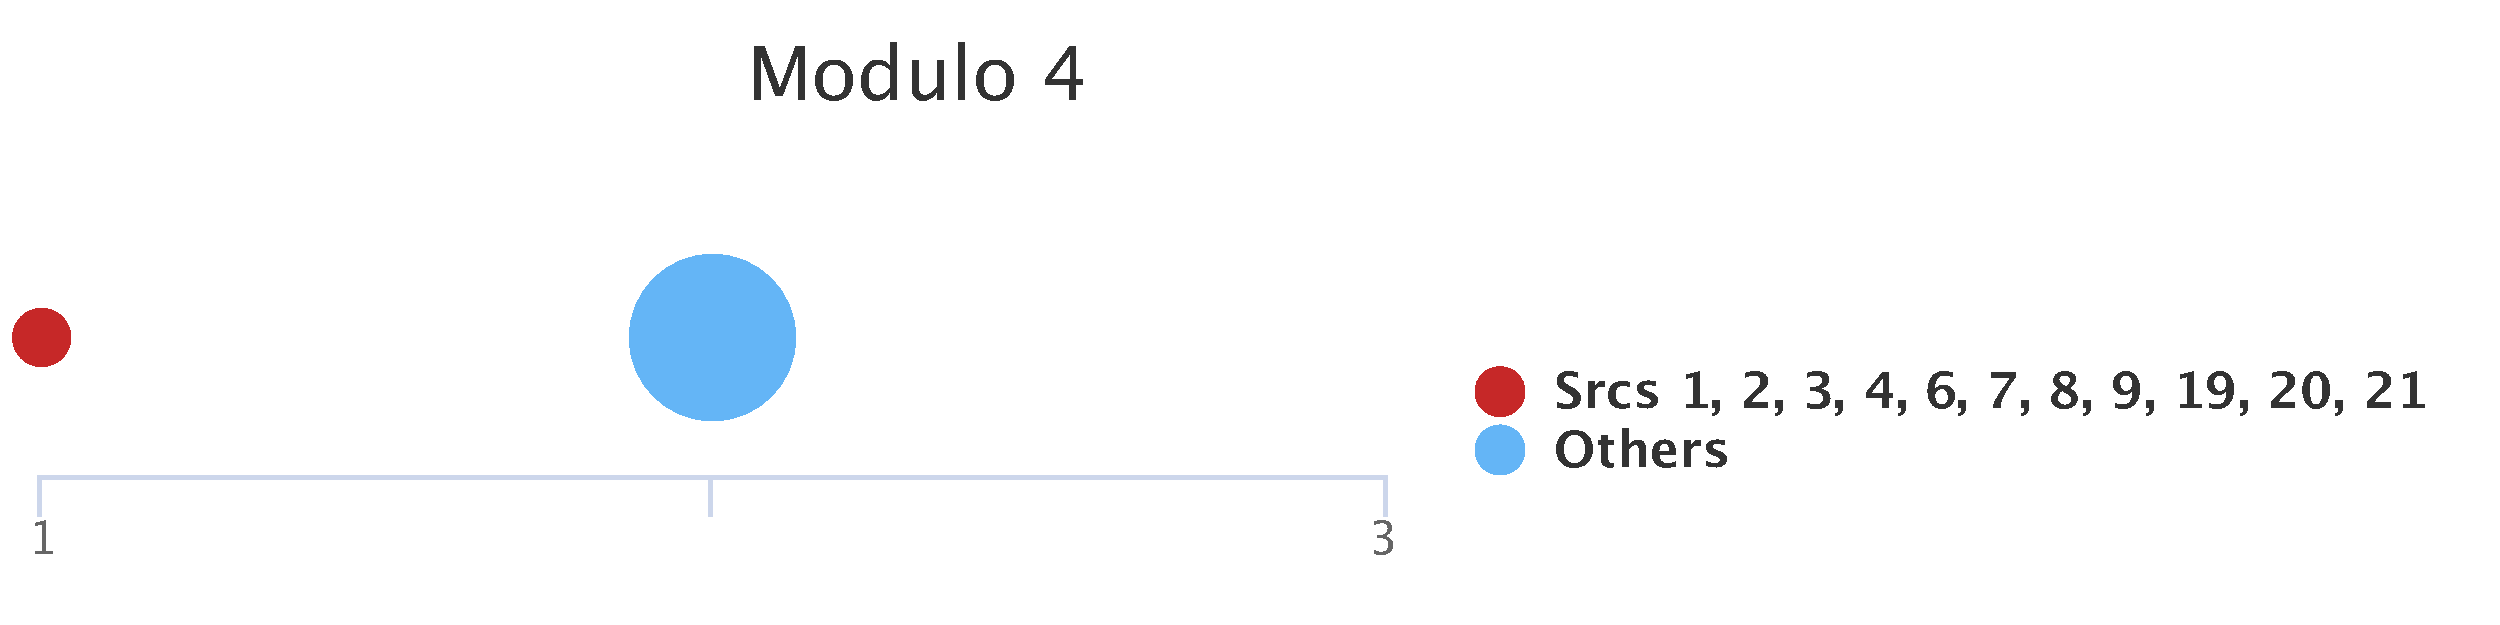
\includegraphics[width=\linewidth]{tex/images/analysis/mod4}
\end{subfigure}\\

\begin{subfigure}{0.45\textwidth}
	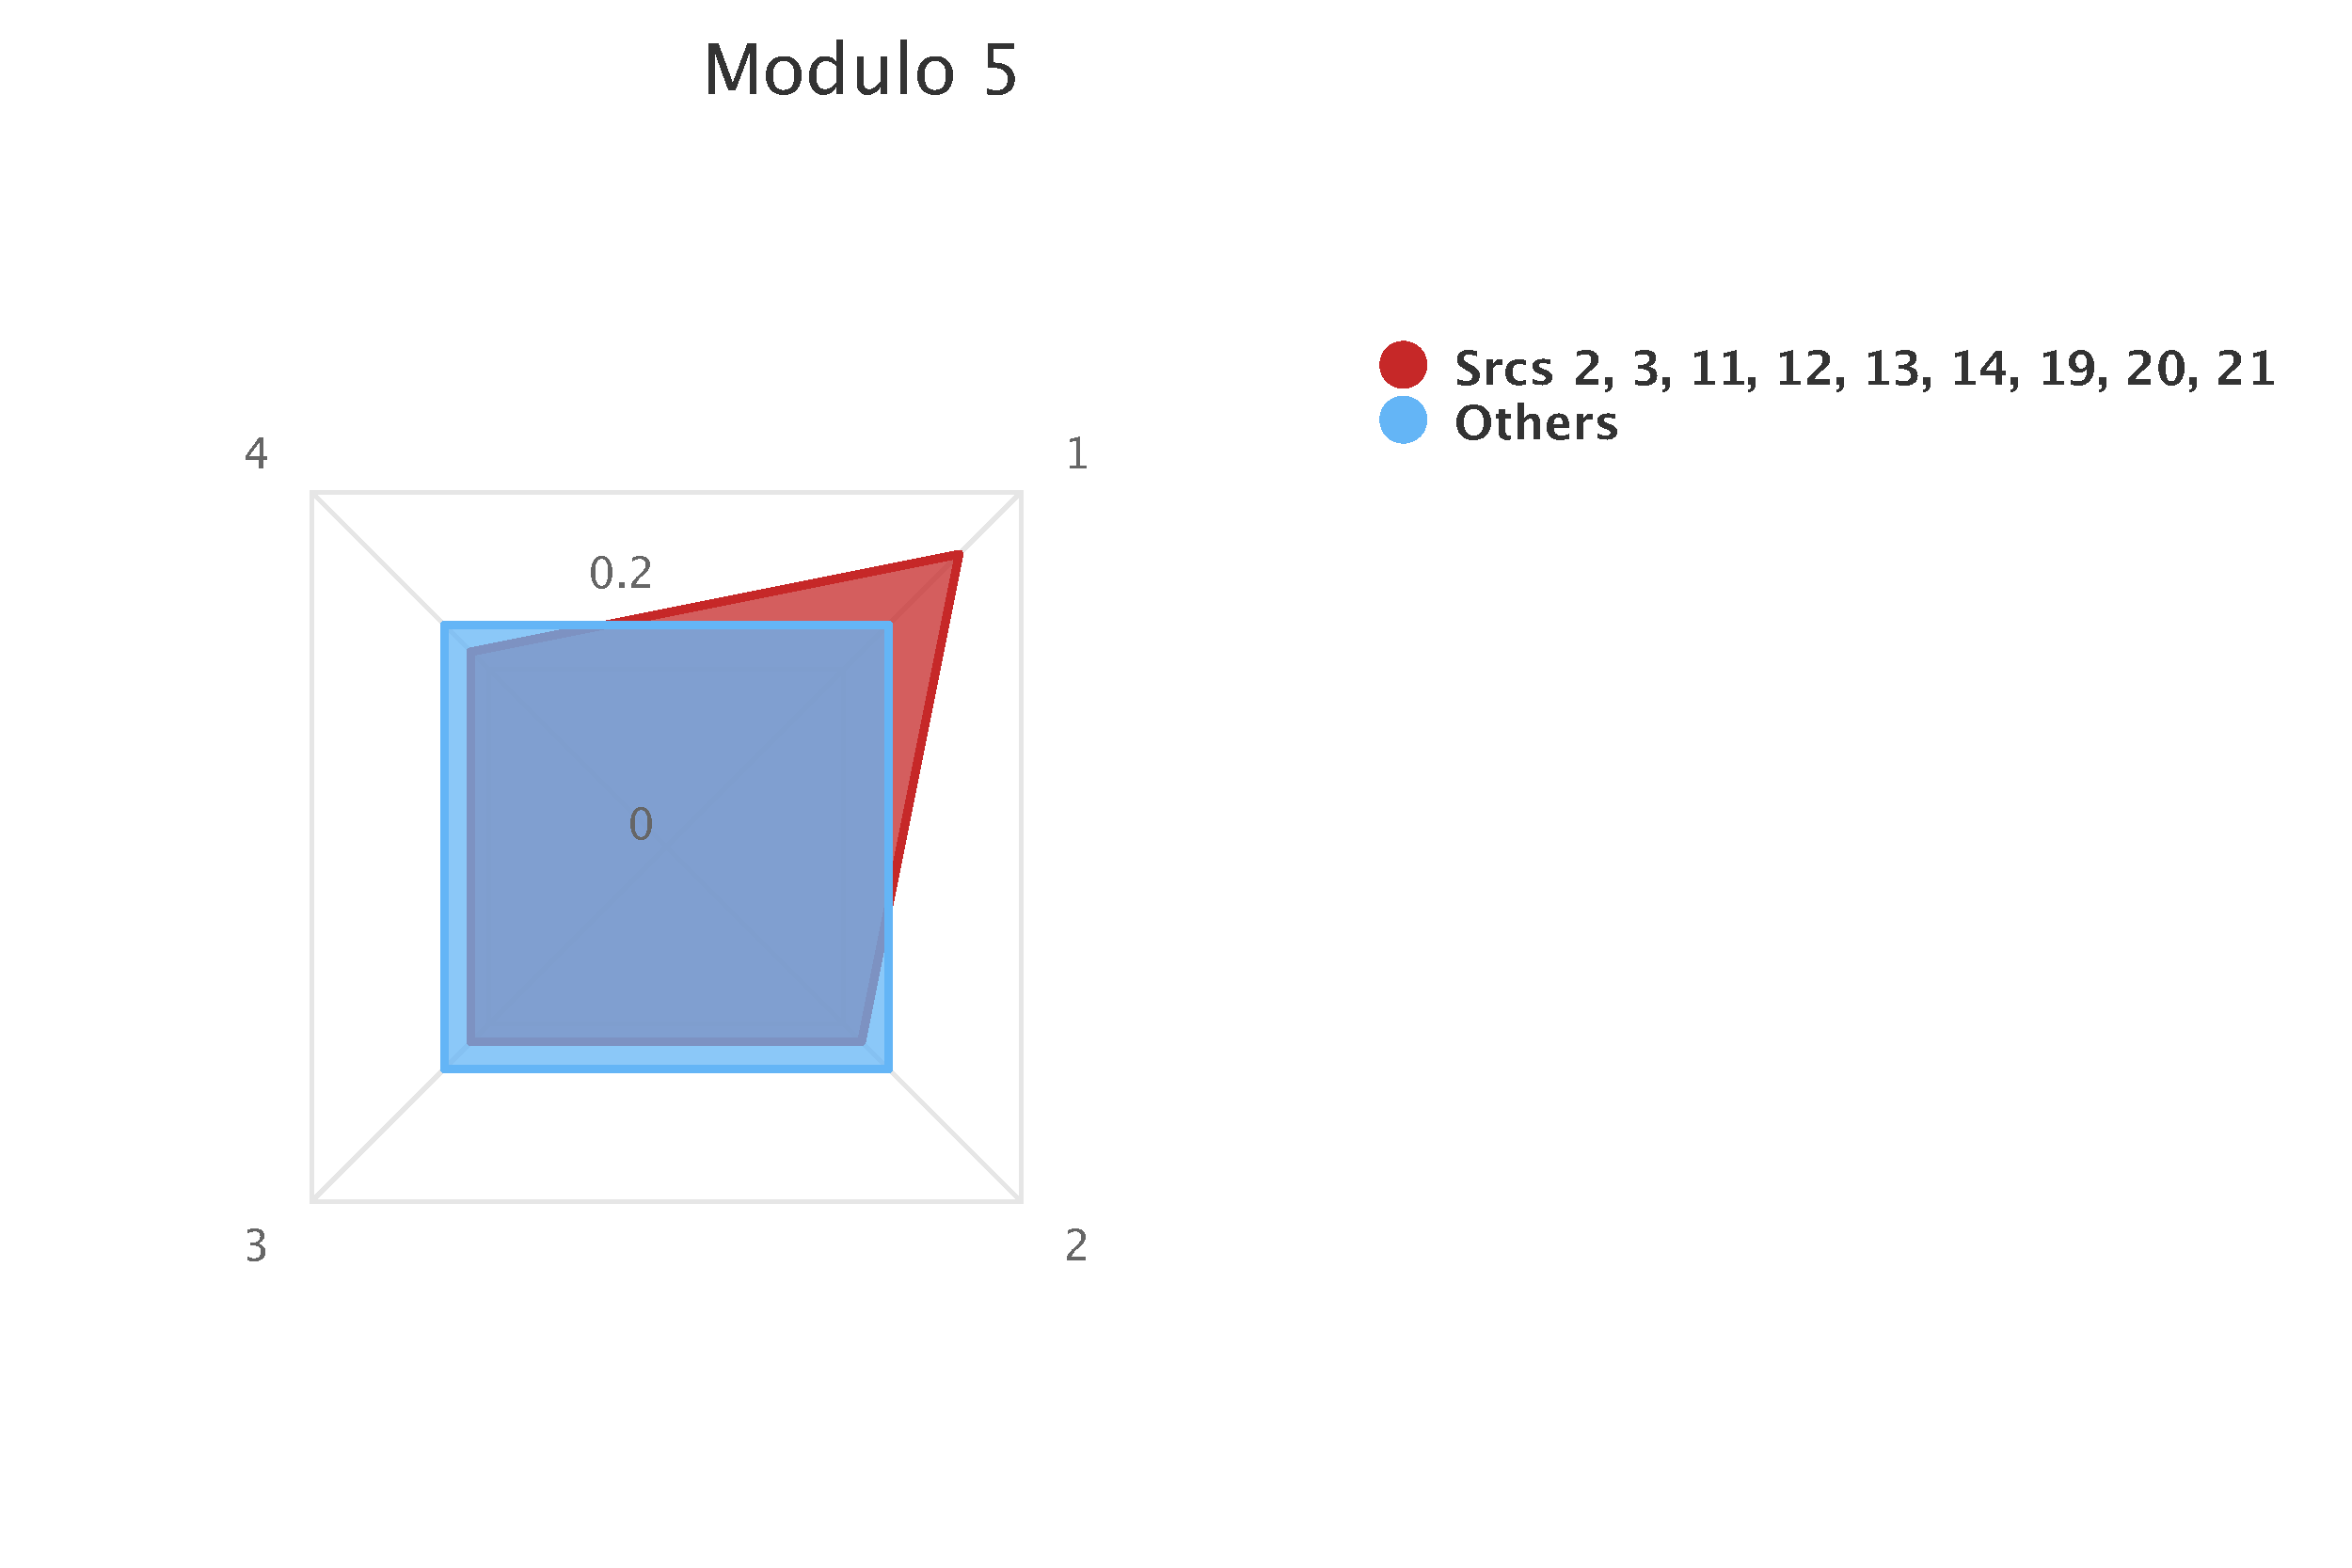
\includegraphics[width=\linewidth]{tex/images/analysis/mod5}
\end{subfigure}
\hfill
\begin{subfigure}{0.45\textwidth}
	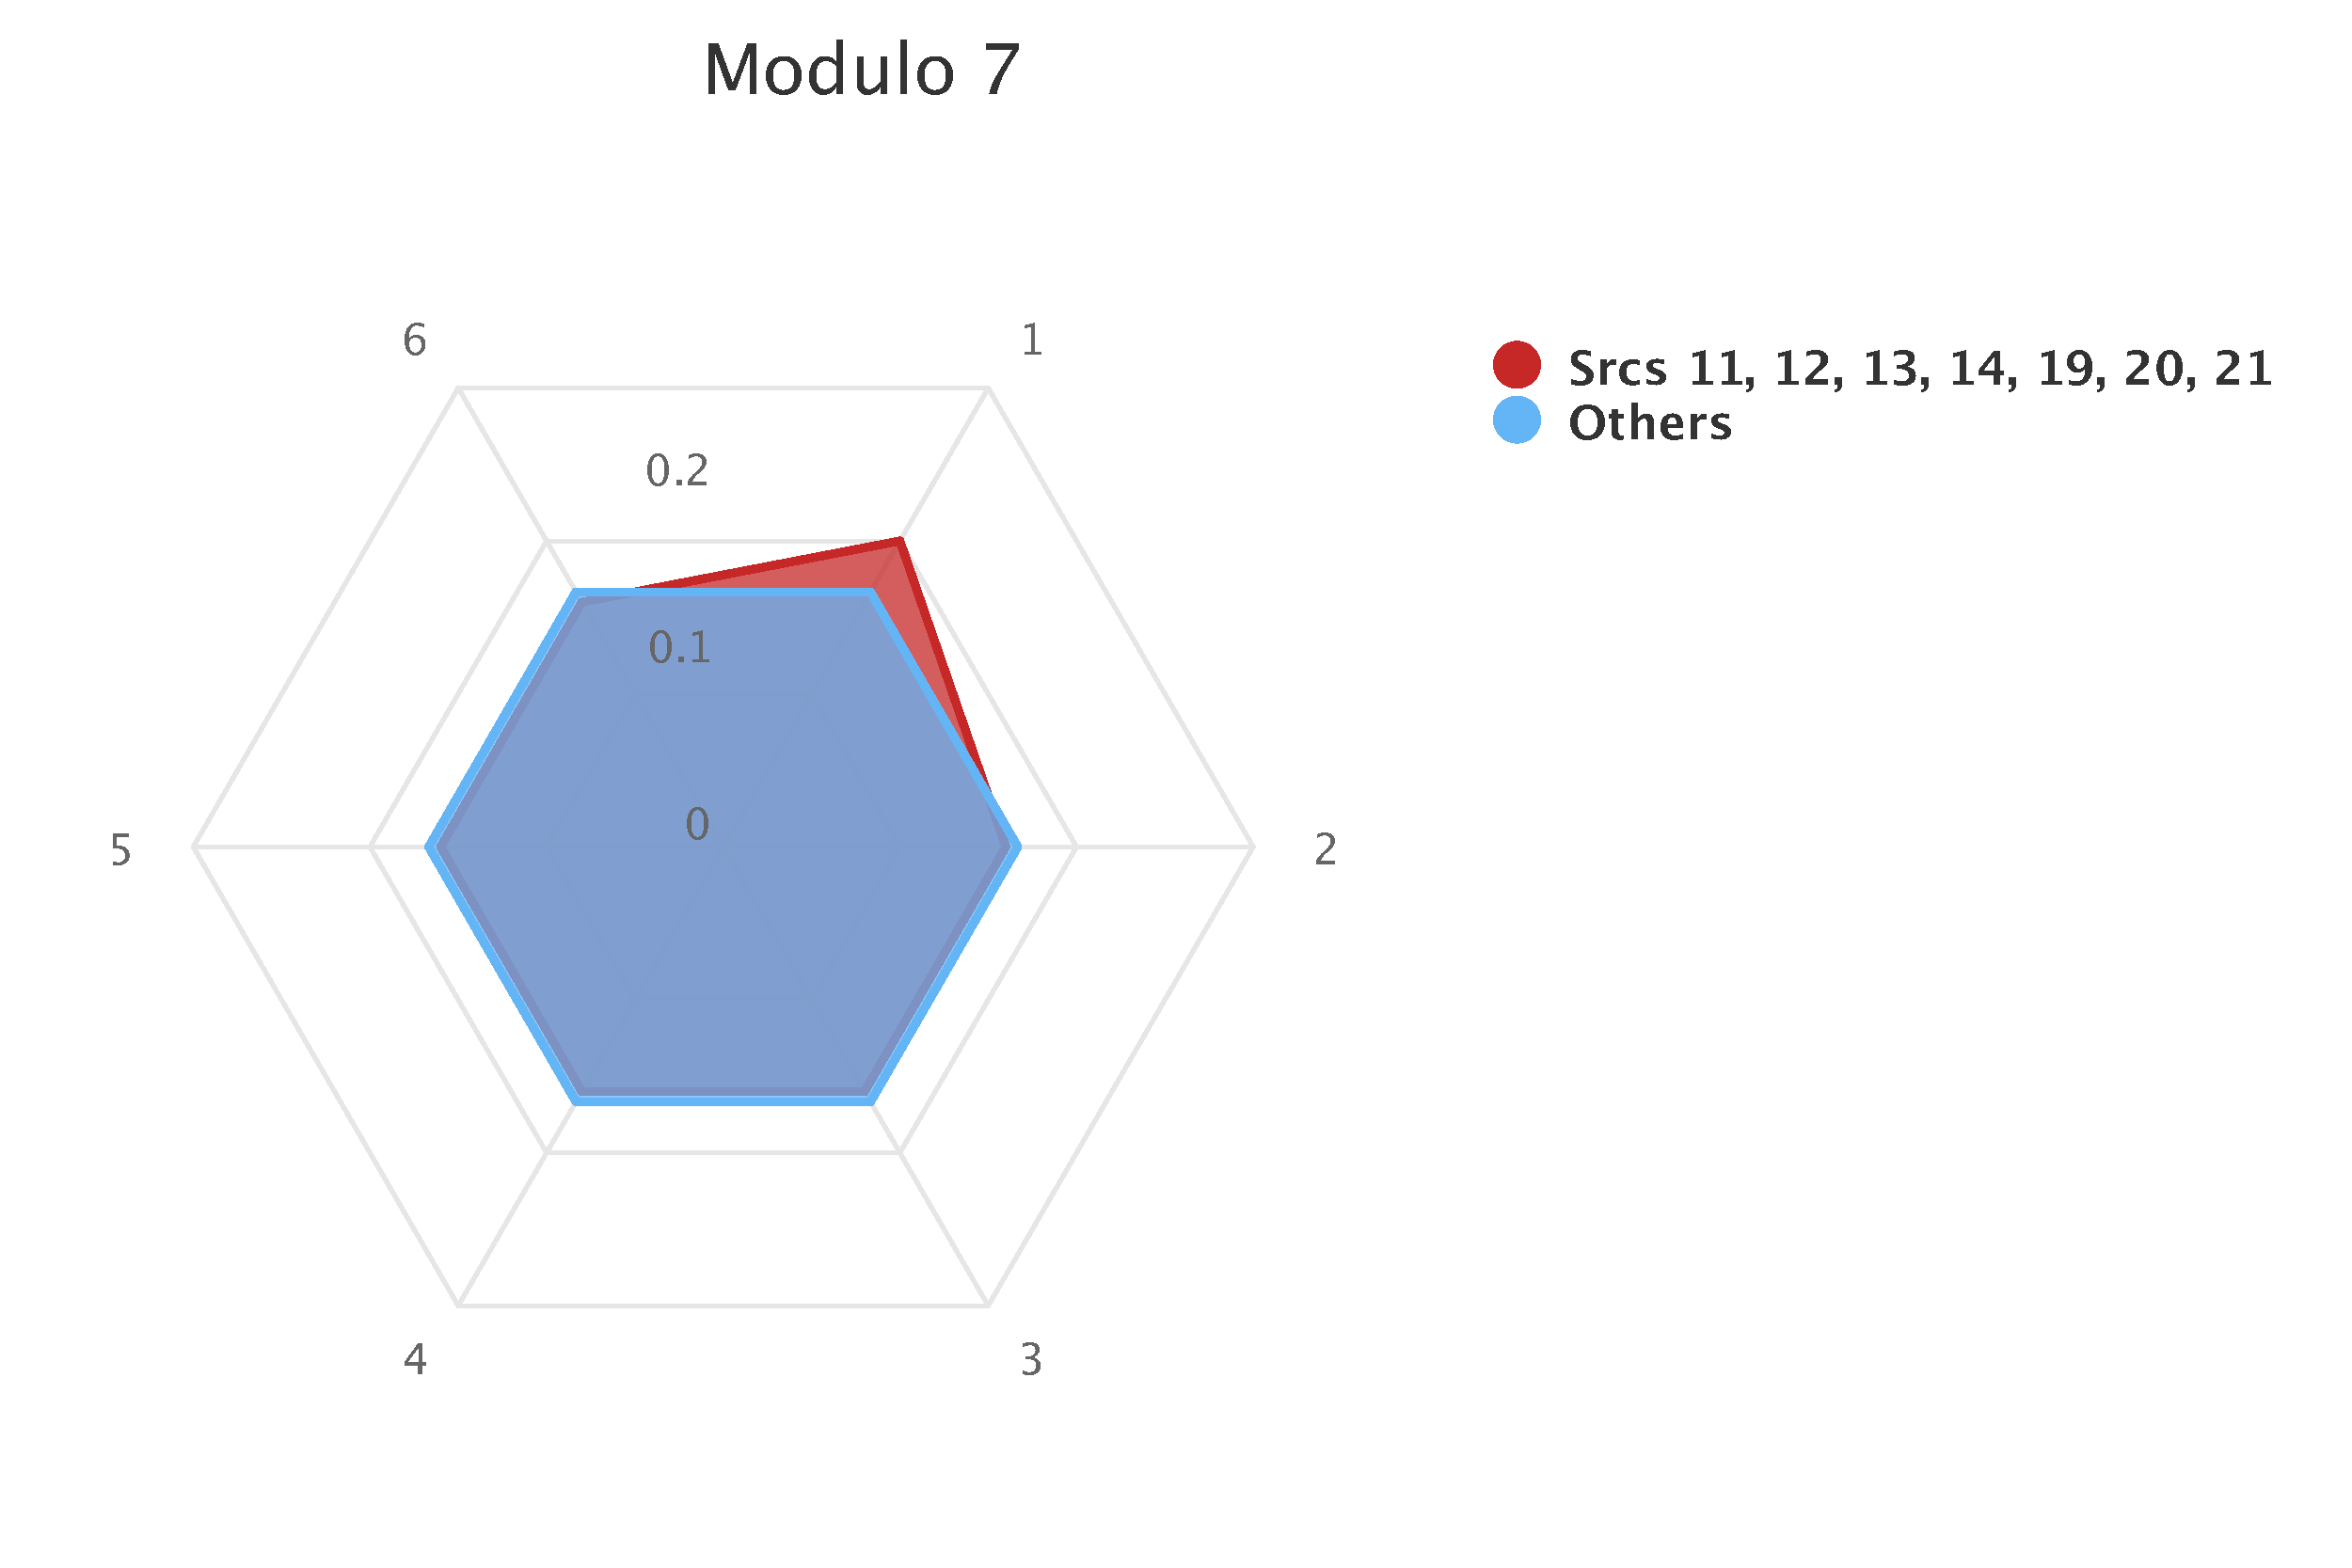
\includegraphics[width=\linewidth]{tex/images/analysis/mod7}
\end{subfigure}\\

\begin{subfigure}{0.45\textwidth}
	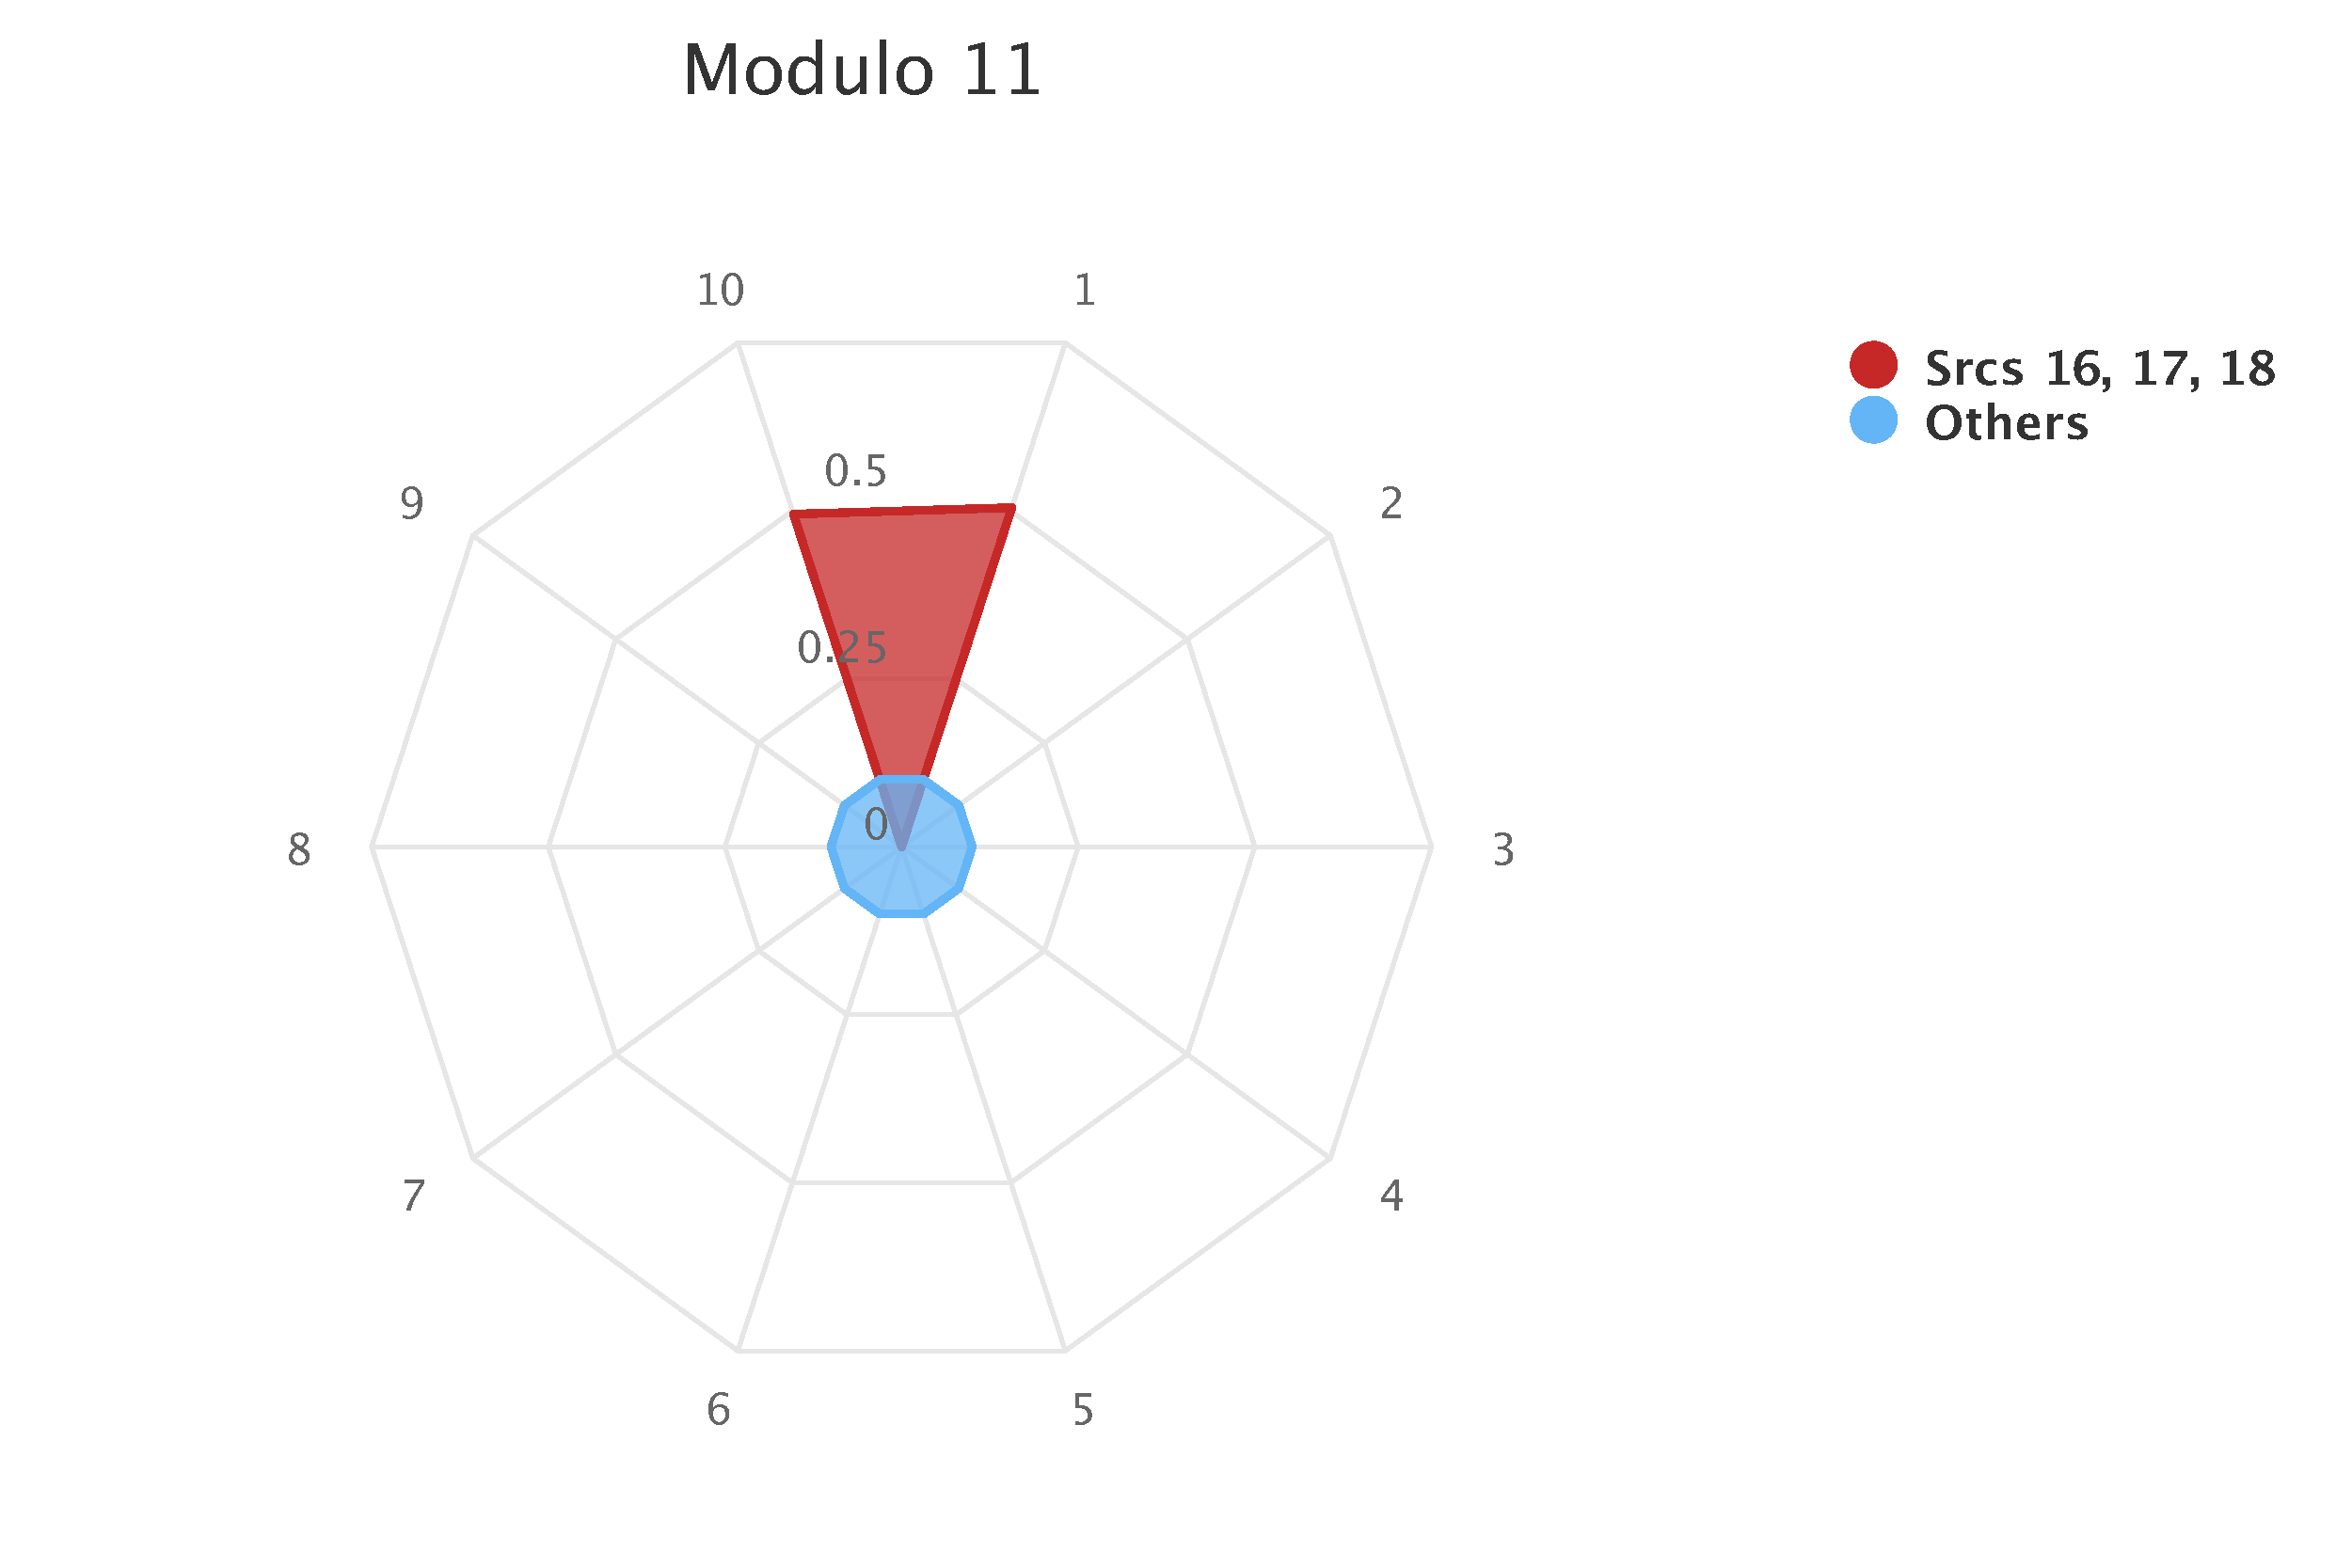
\includegraphics[width=\linewidth]{tex/images/analysis/mod11}
\end{subfigure}
\hfill
\begin{subfigure}{0.45\textwidth}
	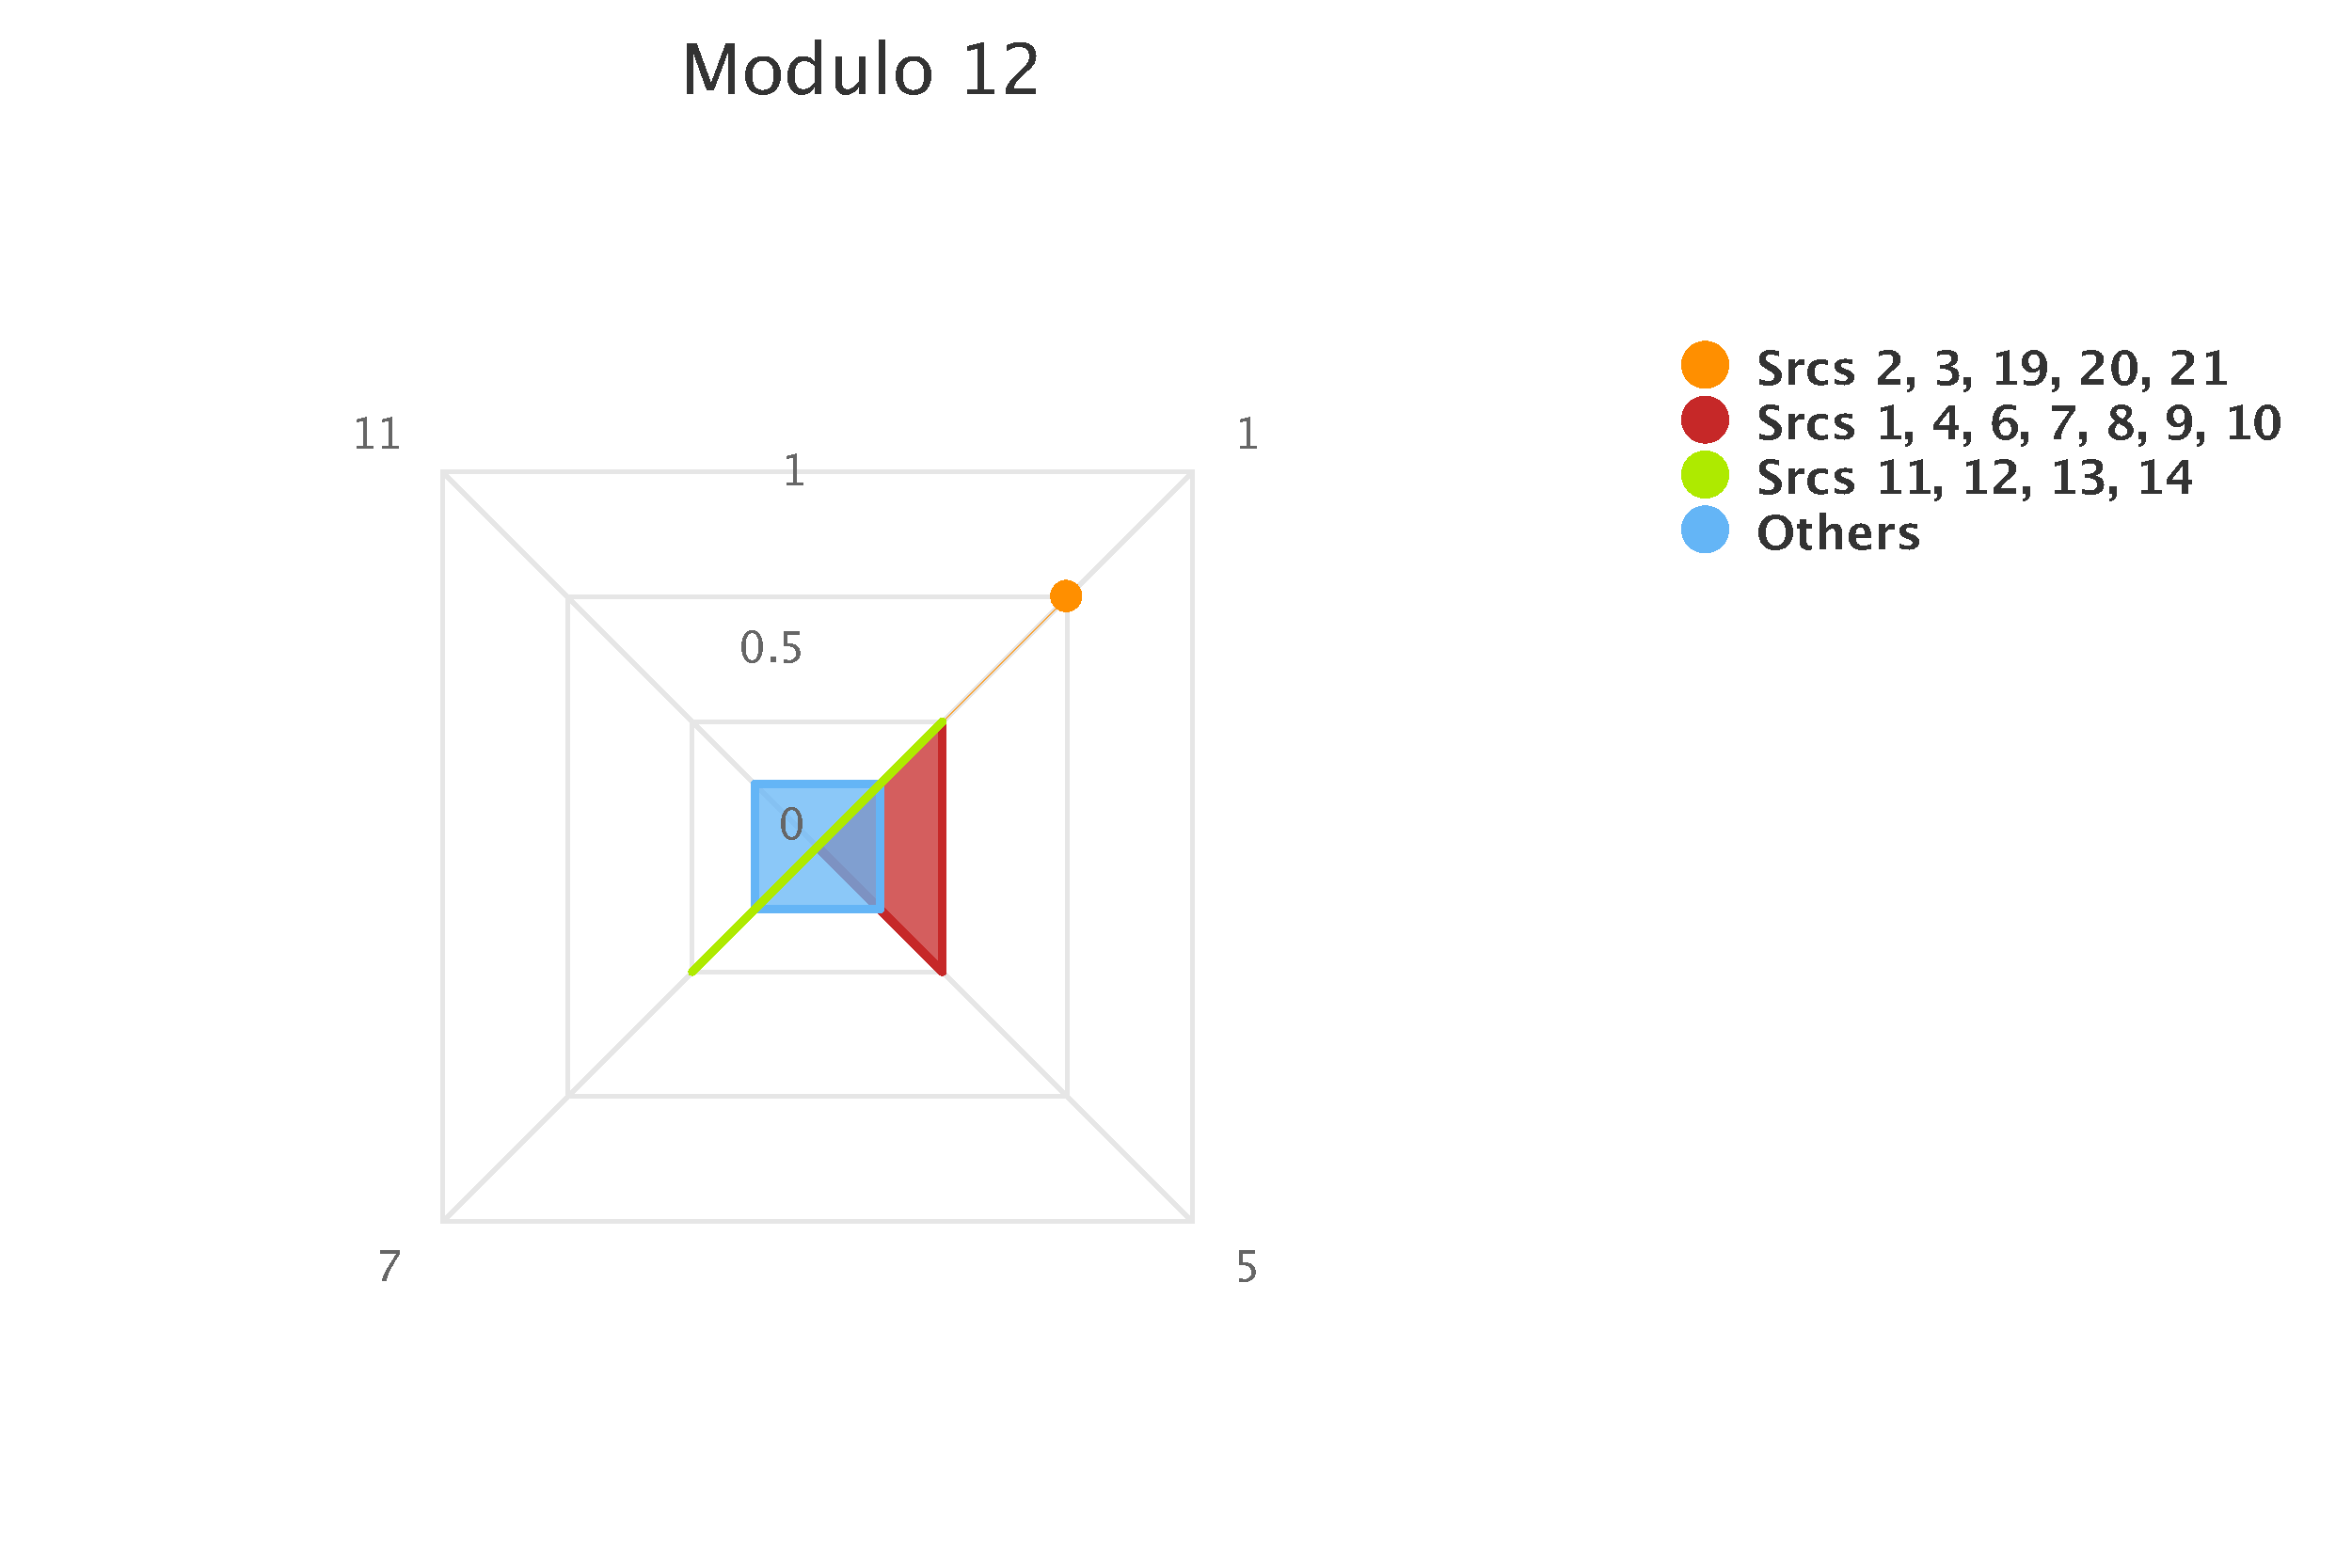
\includegraphics[width=\linewidth]{tex/images/analysis/mod12}
\end{subfigure}\\

\begin{subfigure}{0.45\textwidth}
	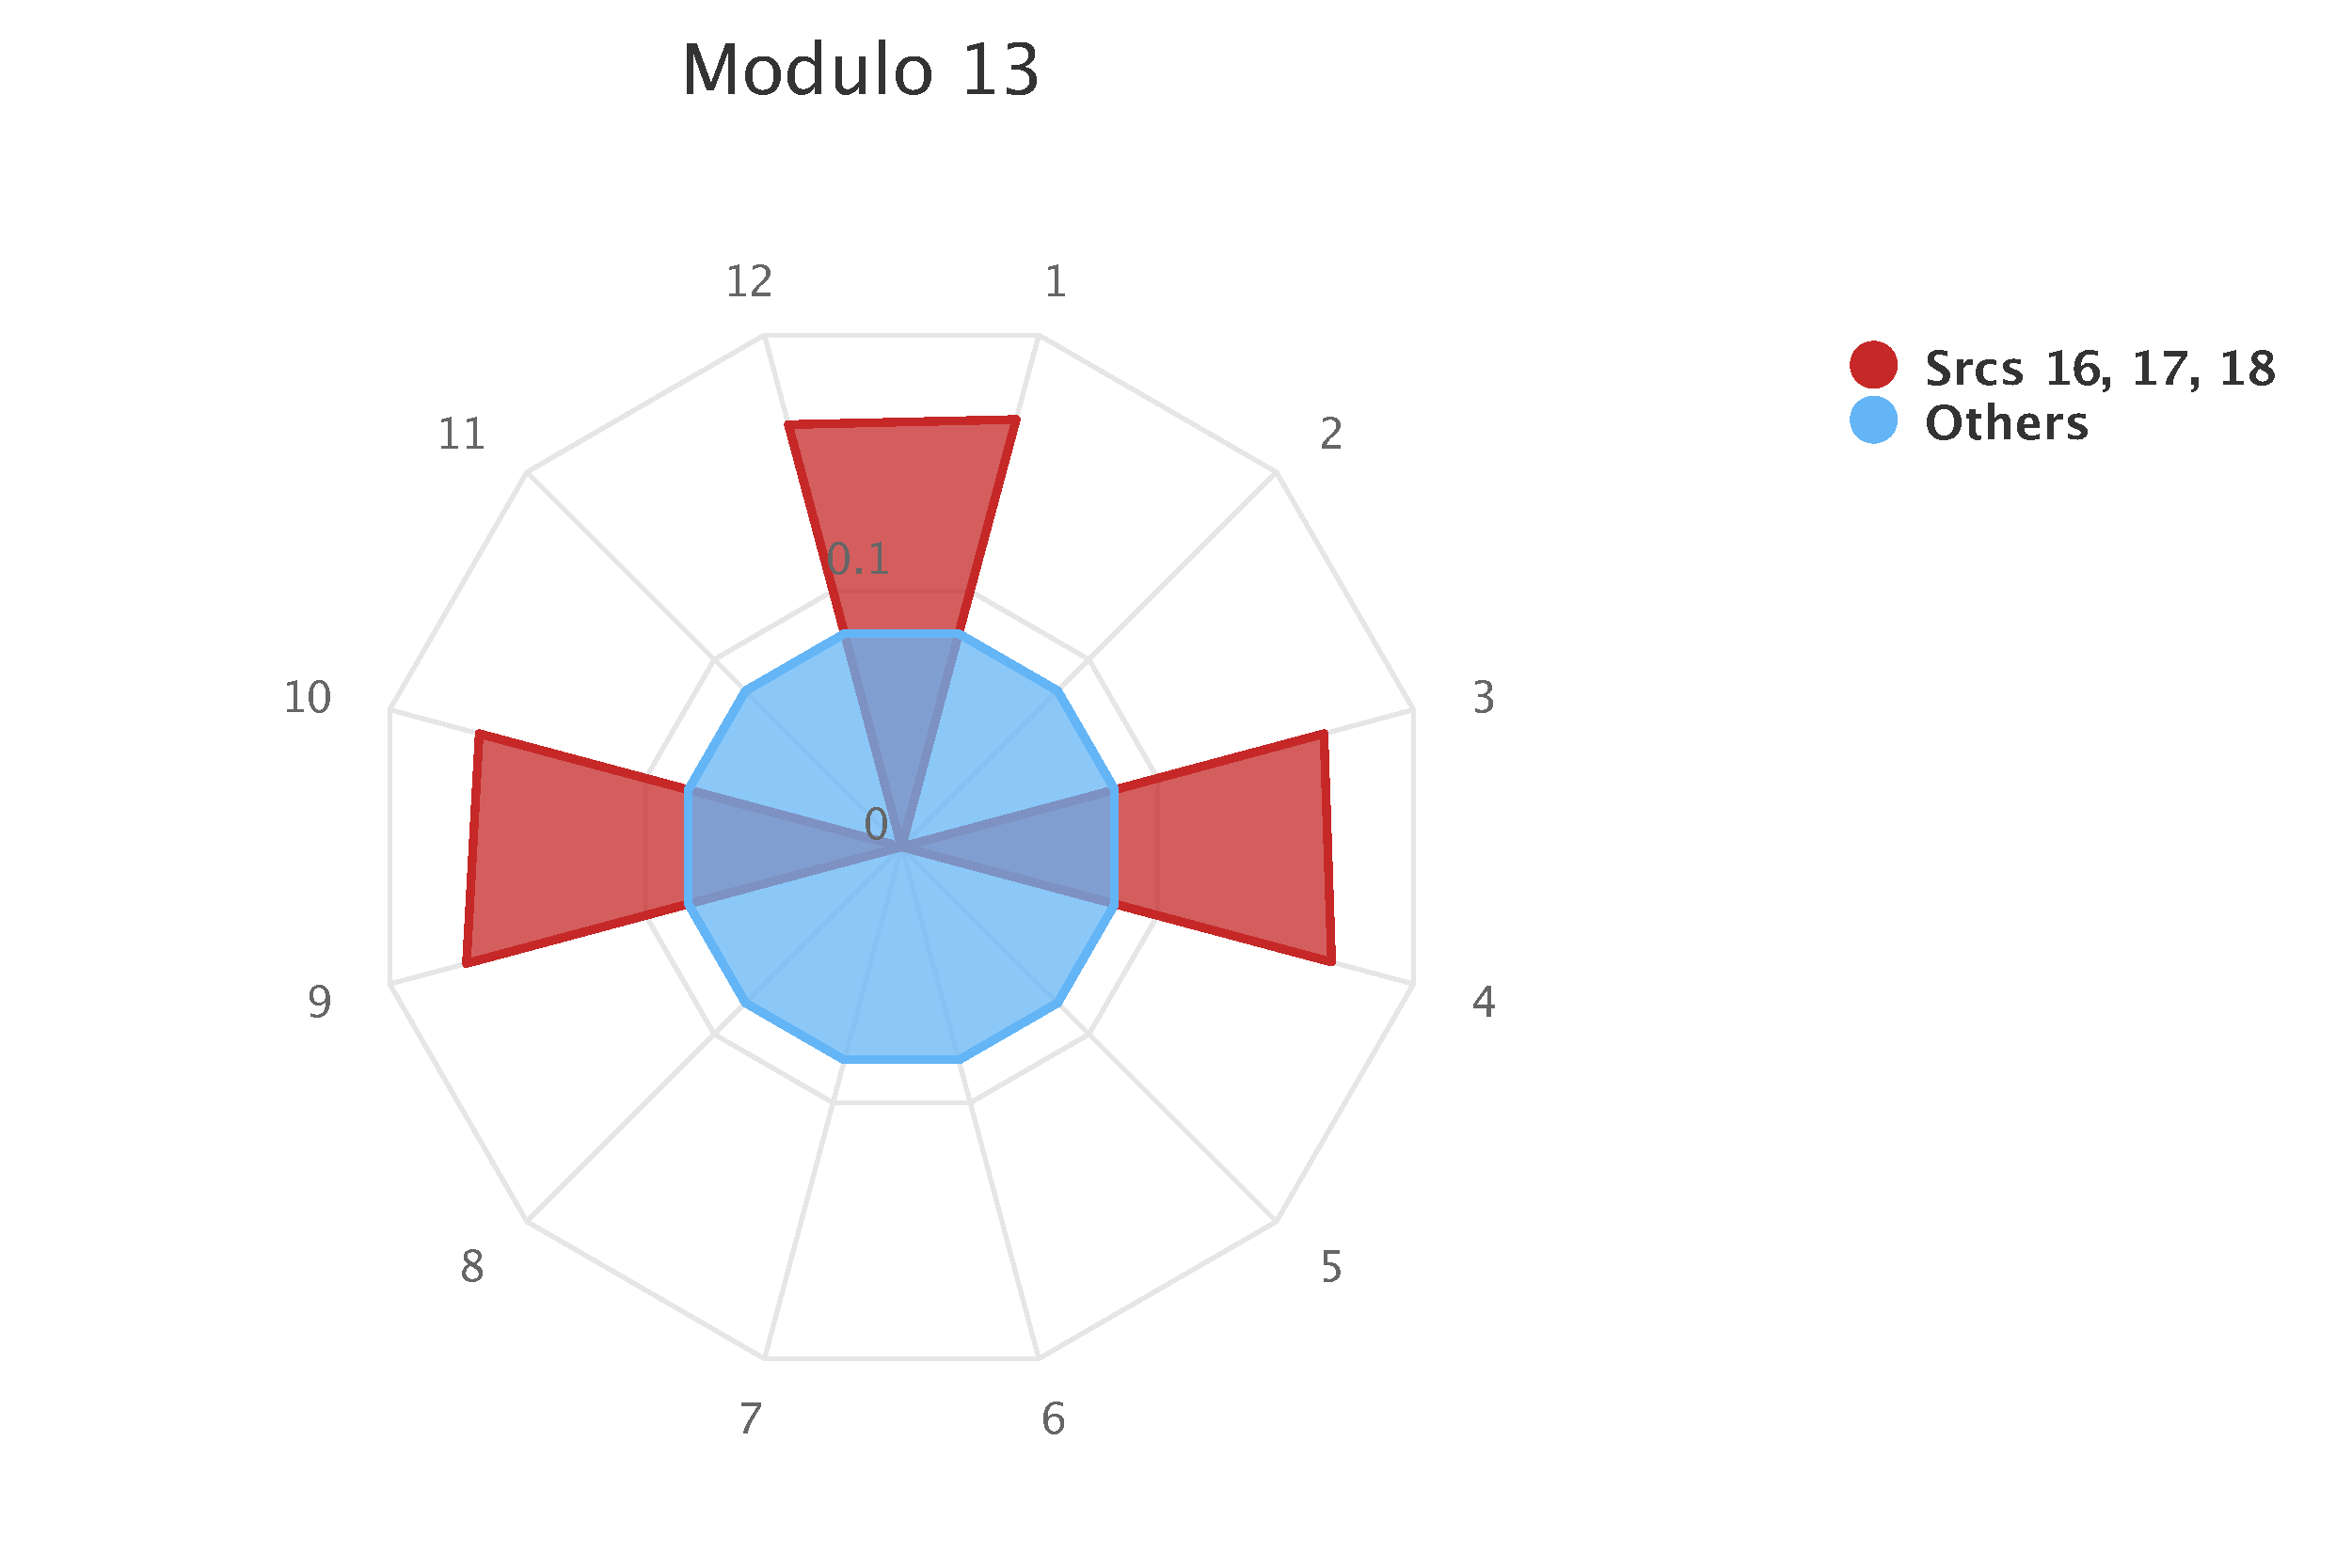
\includegraphics[width=\linewidth]{tex/images/analysis/mod13}
\end{subfigure}
\hfill
\begin{subfigure}{0.45\textwidth}
	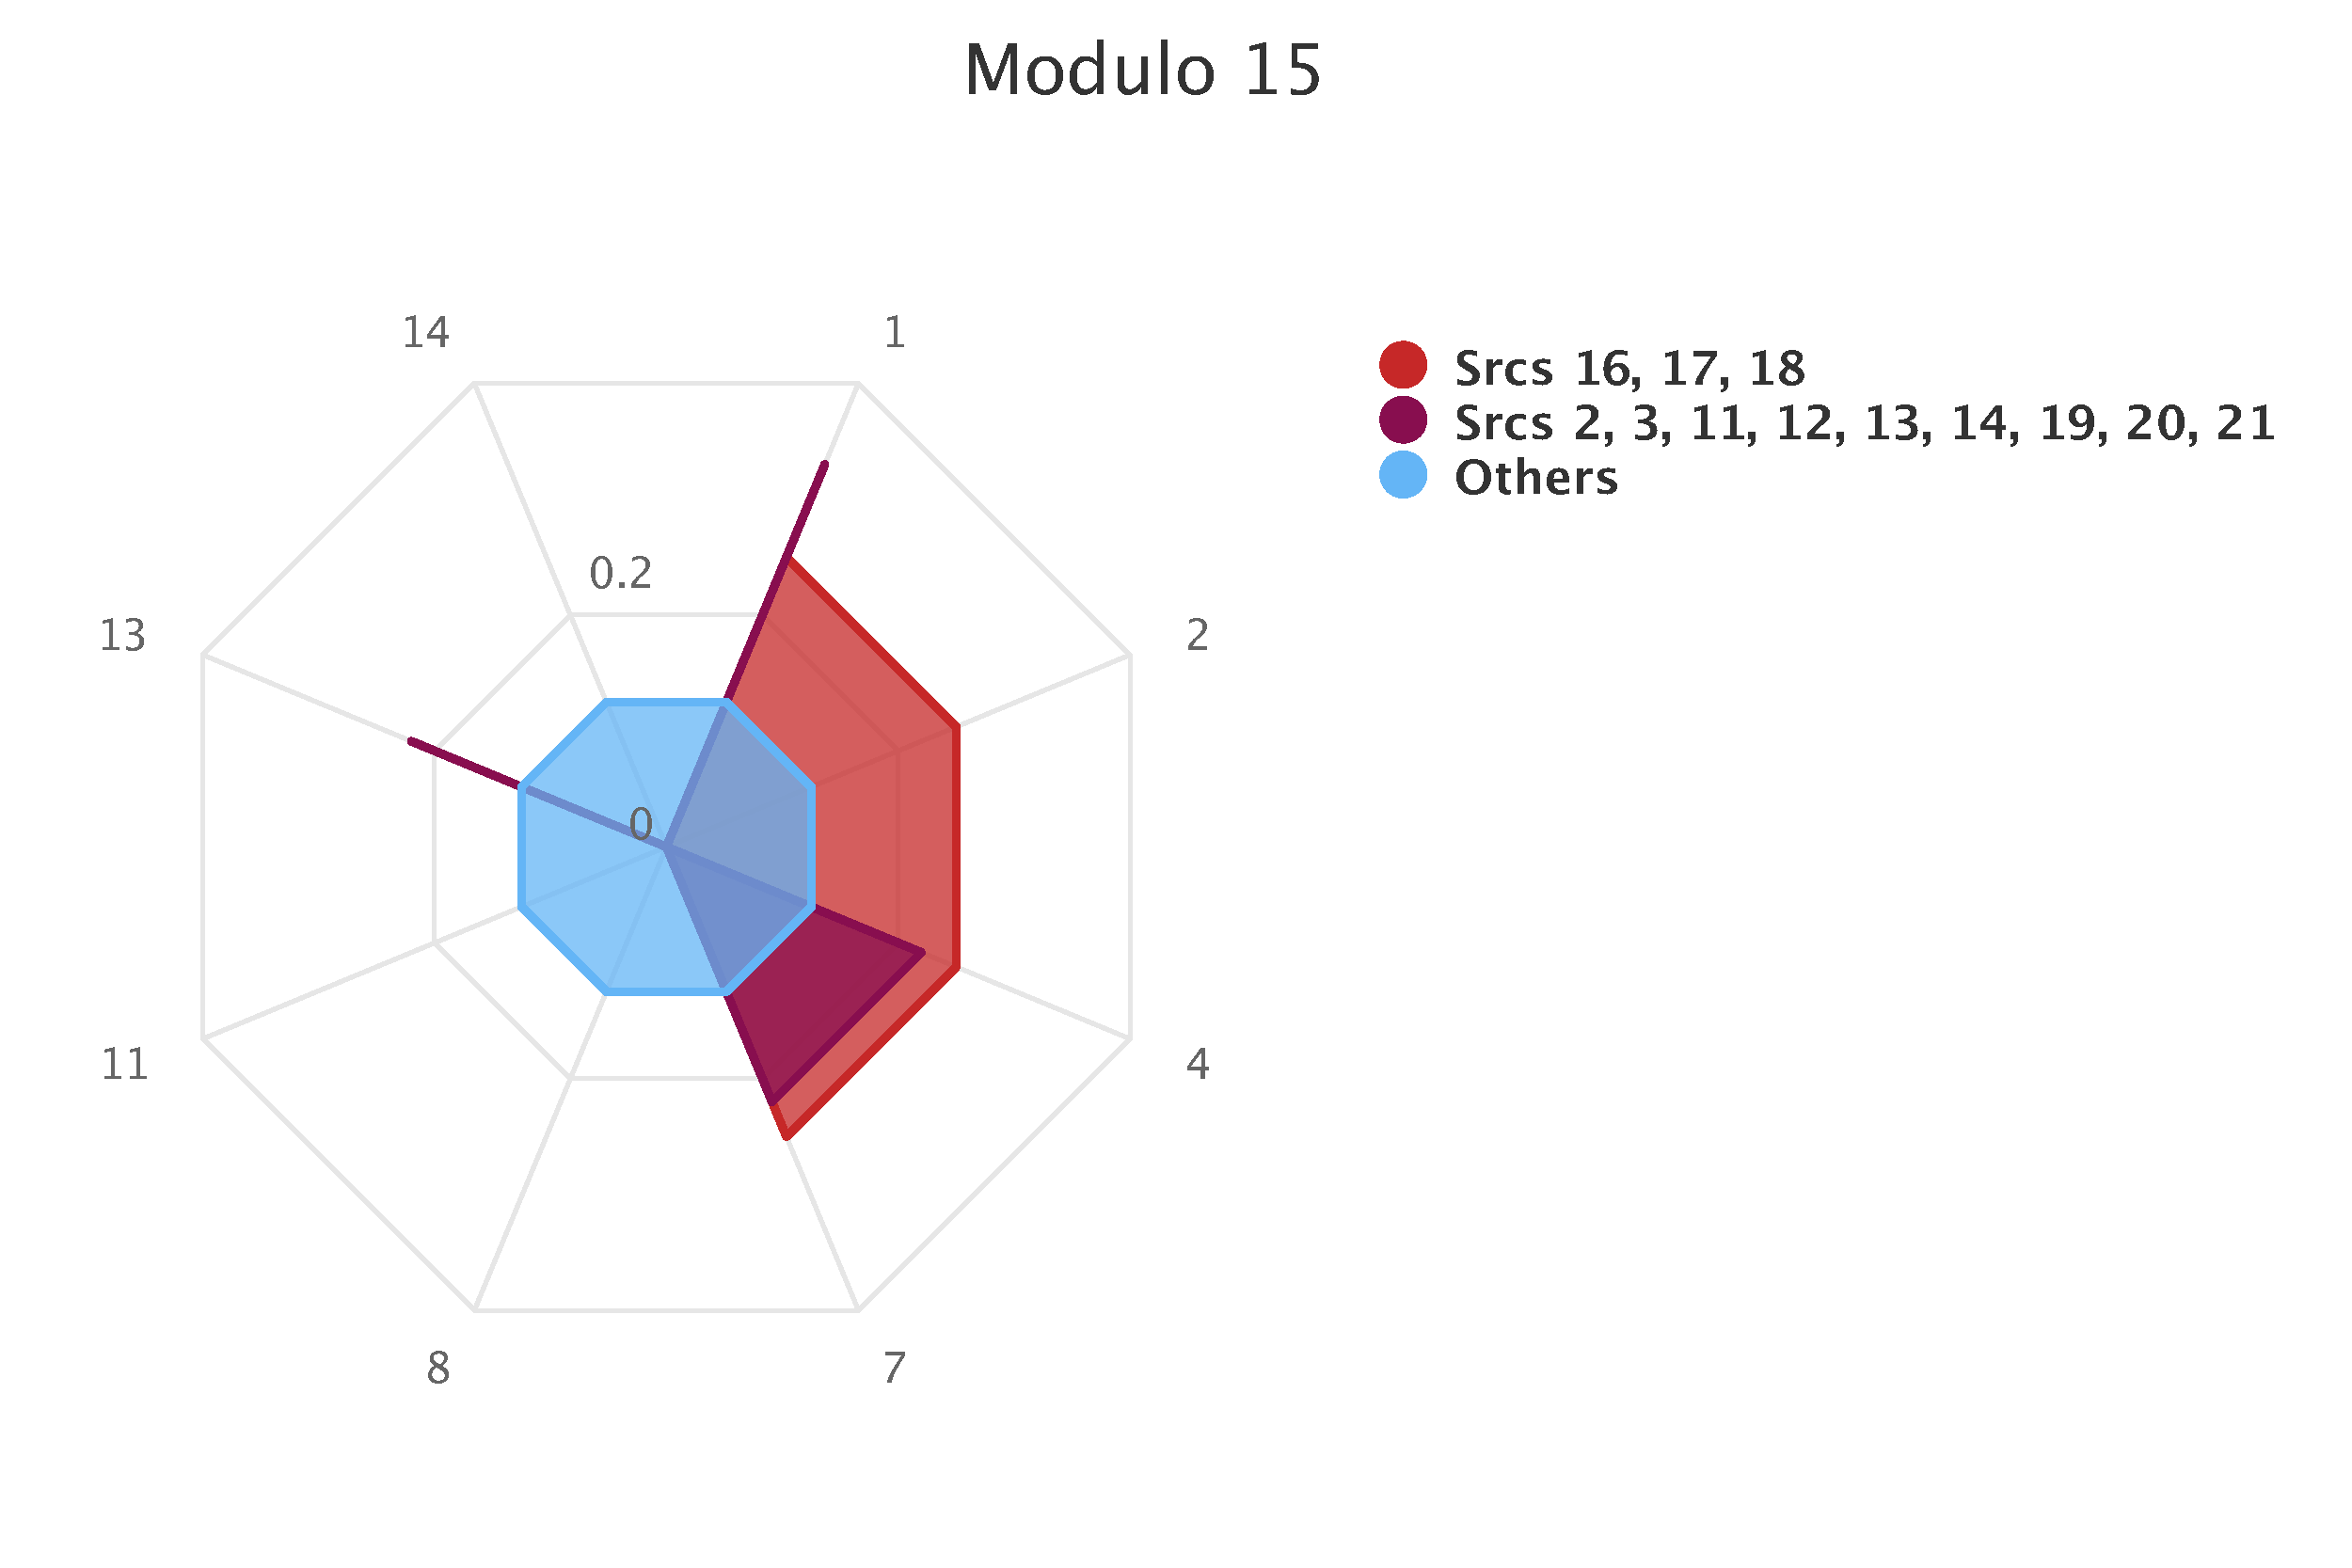
\includegraphics[width=\linewidth]{tex/images/analysis/mod15}
\end{subfigure}\\

\caption{Modular bias visualization, the following radar charts show the individual possible remainders. The blue area represents the uniform distribution, which includes most of the sources. The other colors are non-uniform distributions found in some sources. For example, sources 11-14, 19, 20, 21 are slightly biased towards 1 modulo 7.}
\end{figure}
\label{figure-mod-analysis}

\begin{figure}[H]
\centering
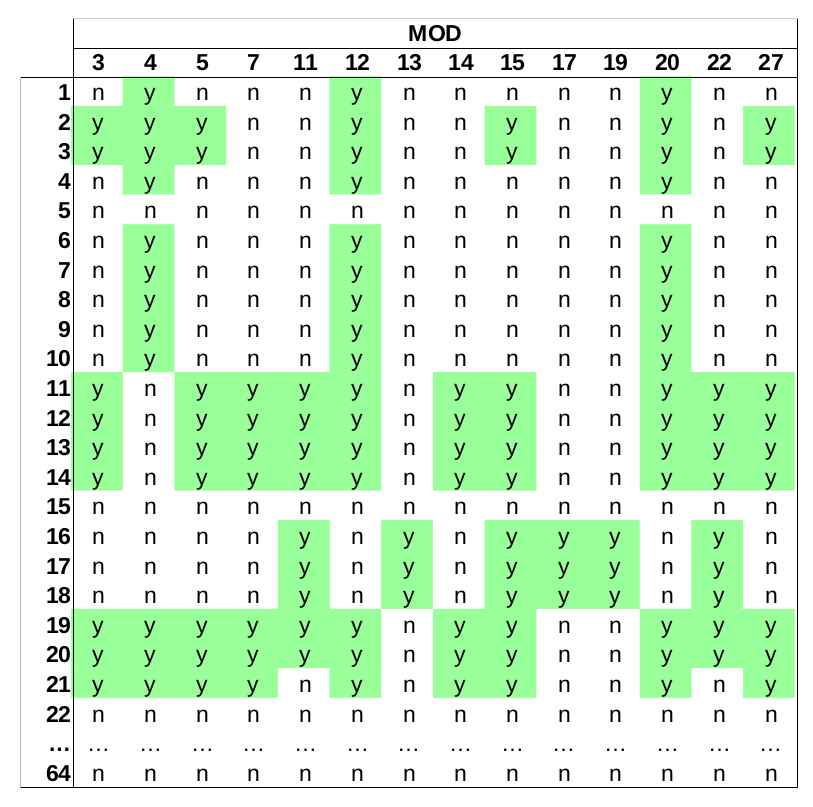
\includegraphics[width=0.64\textwidth]{tex/images/mod_analysis}
\caption{Table of biases. For sources 5, 15, 22-64 no biases have been found.}

\end{figure}

\newpage

\section{Bit analysis}
\label{appendix-bit-analysis}

\begin{figure}[H]
	\centering
	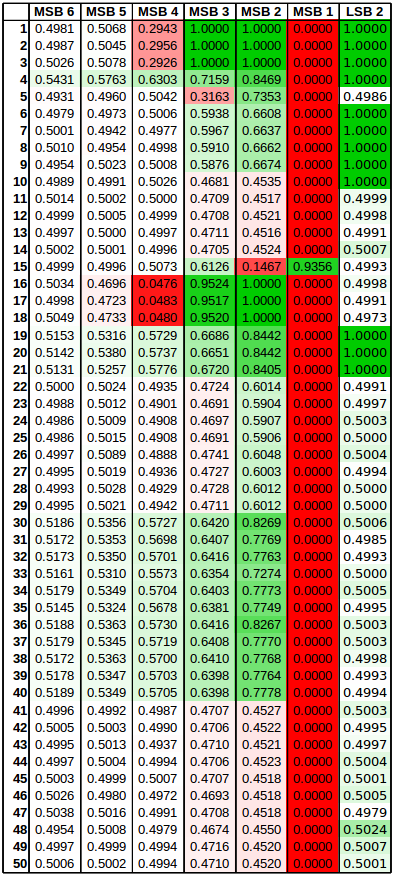
\includegraphics[width=0.64\linewidth]{tex/images/analysis/bit_sheet_1}
\end{figure}

\begin{figure}[H]
	\centering
	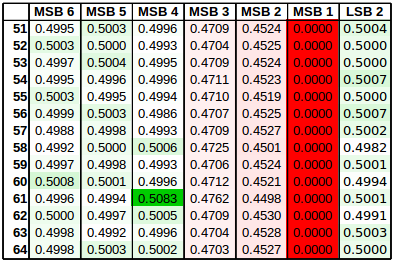
\includegraphics[width=0.64\linewidth]{tex/images/analysis/bit_sheet_2}
	\caption{Table of bit biases. The number represents the probability of 0 for a randomly chosen key.}
	\label{figure-table-bit-analysis}
\end{figure}

\begin{figure}[H]
	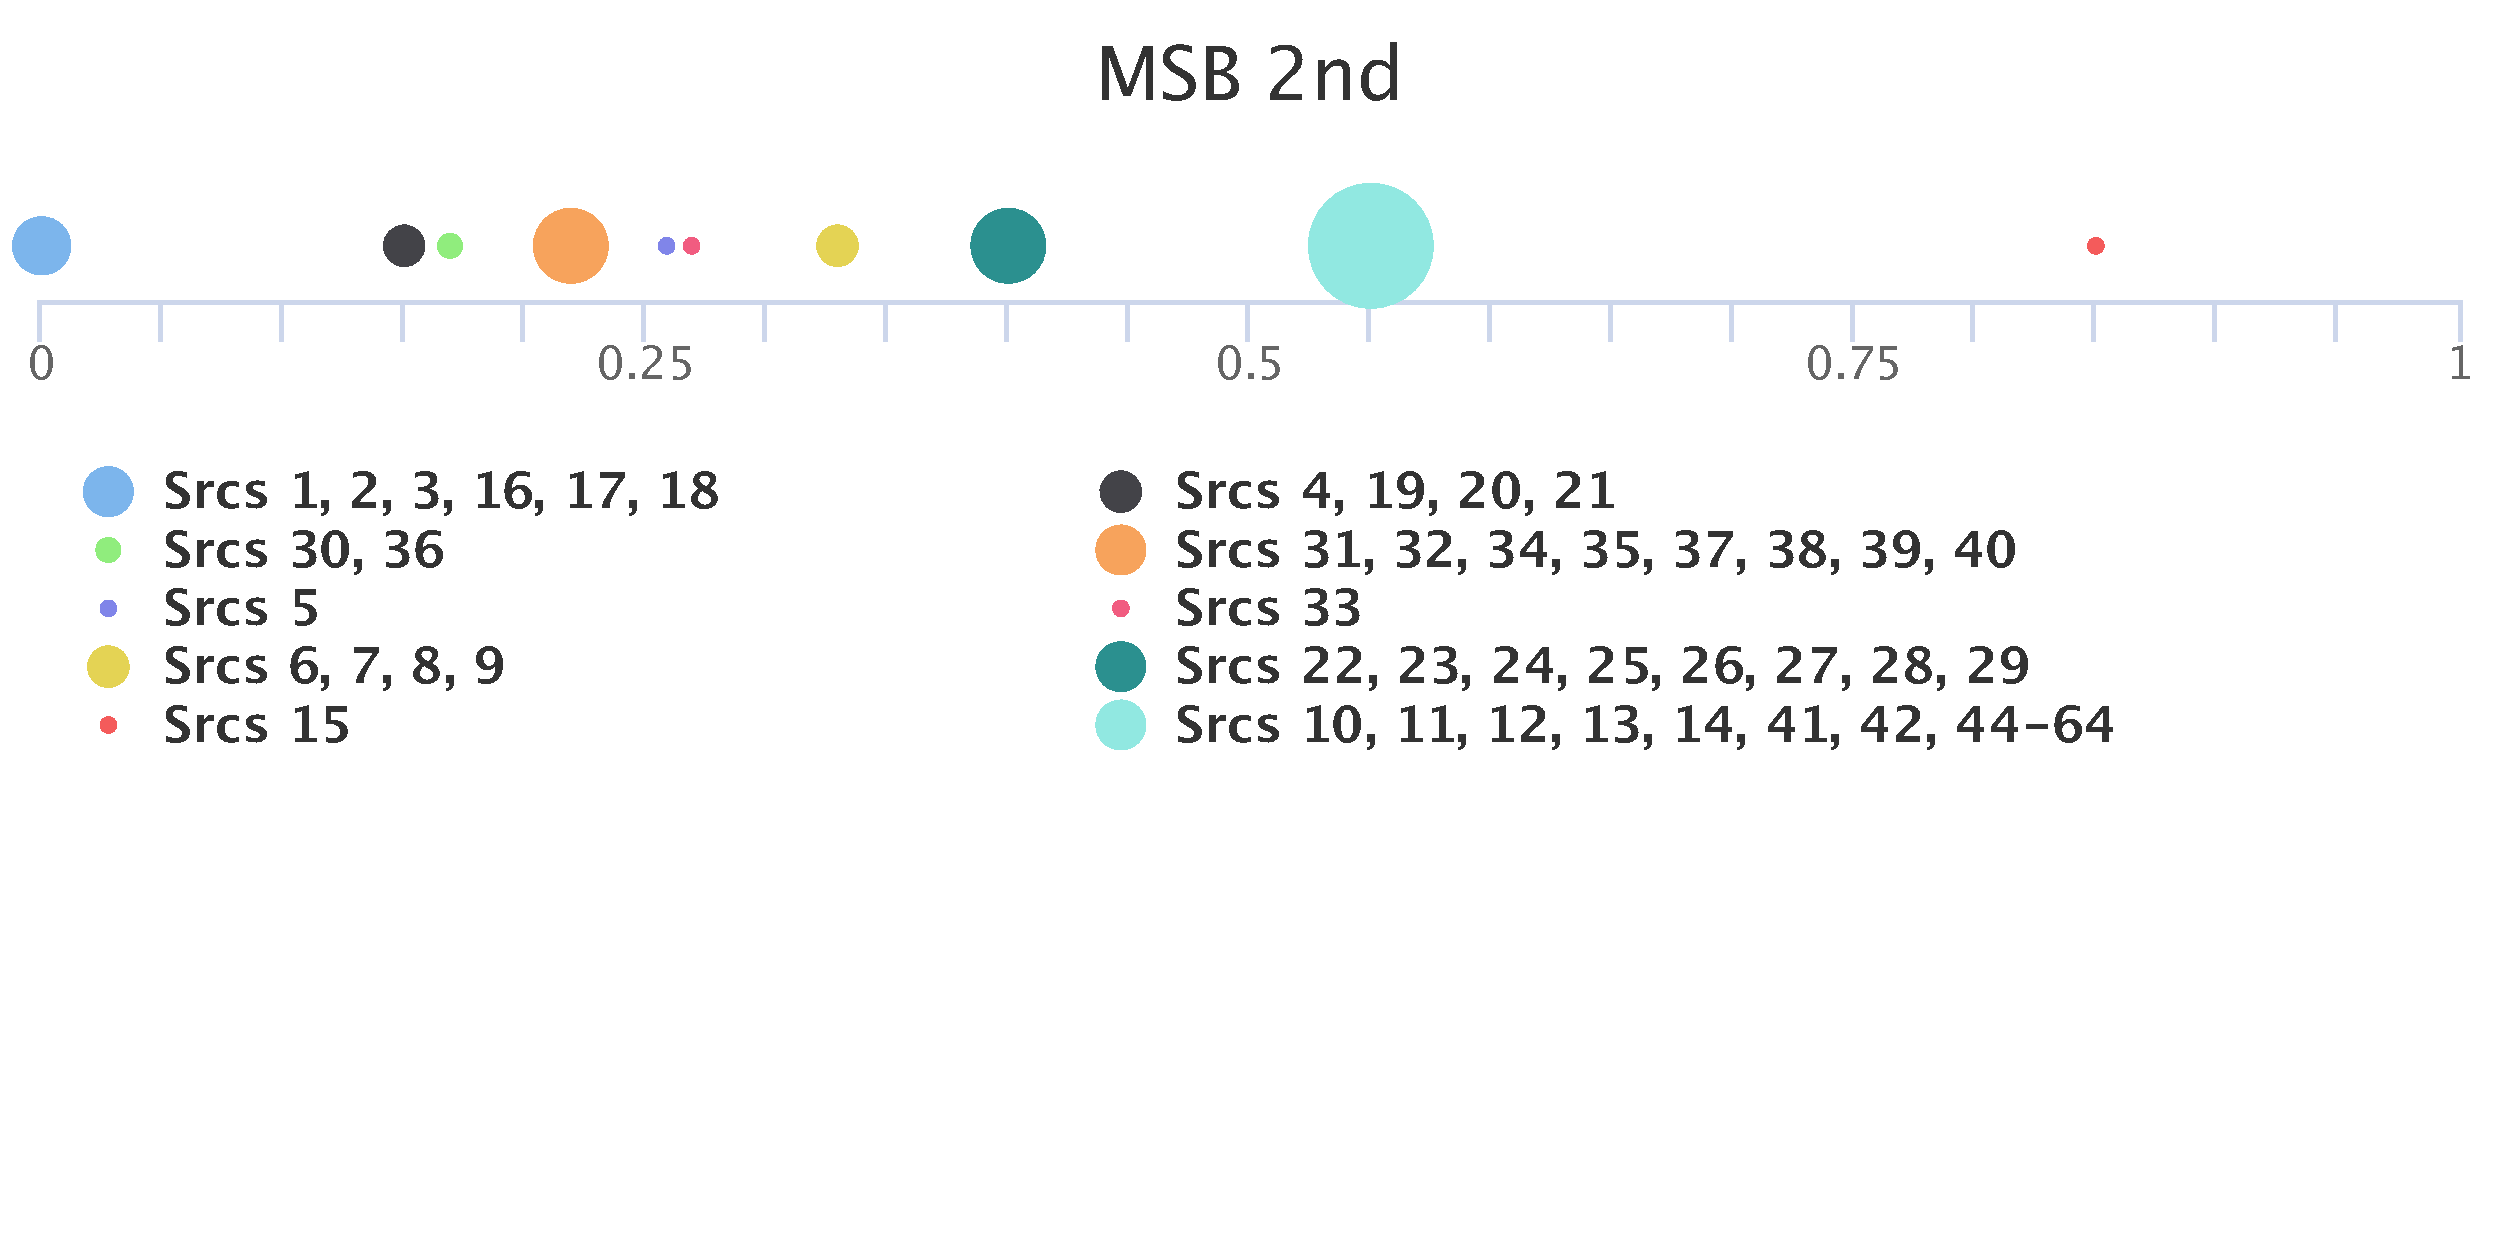
\includegraphics[width=\linewidth]{tex/images/analysis/bit2}
	\caption{Probability of 0 of 2nd most significant bit.}
\end{figure}

\begin{figure}[H]
	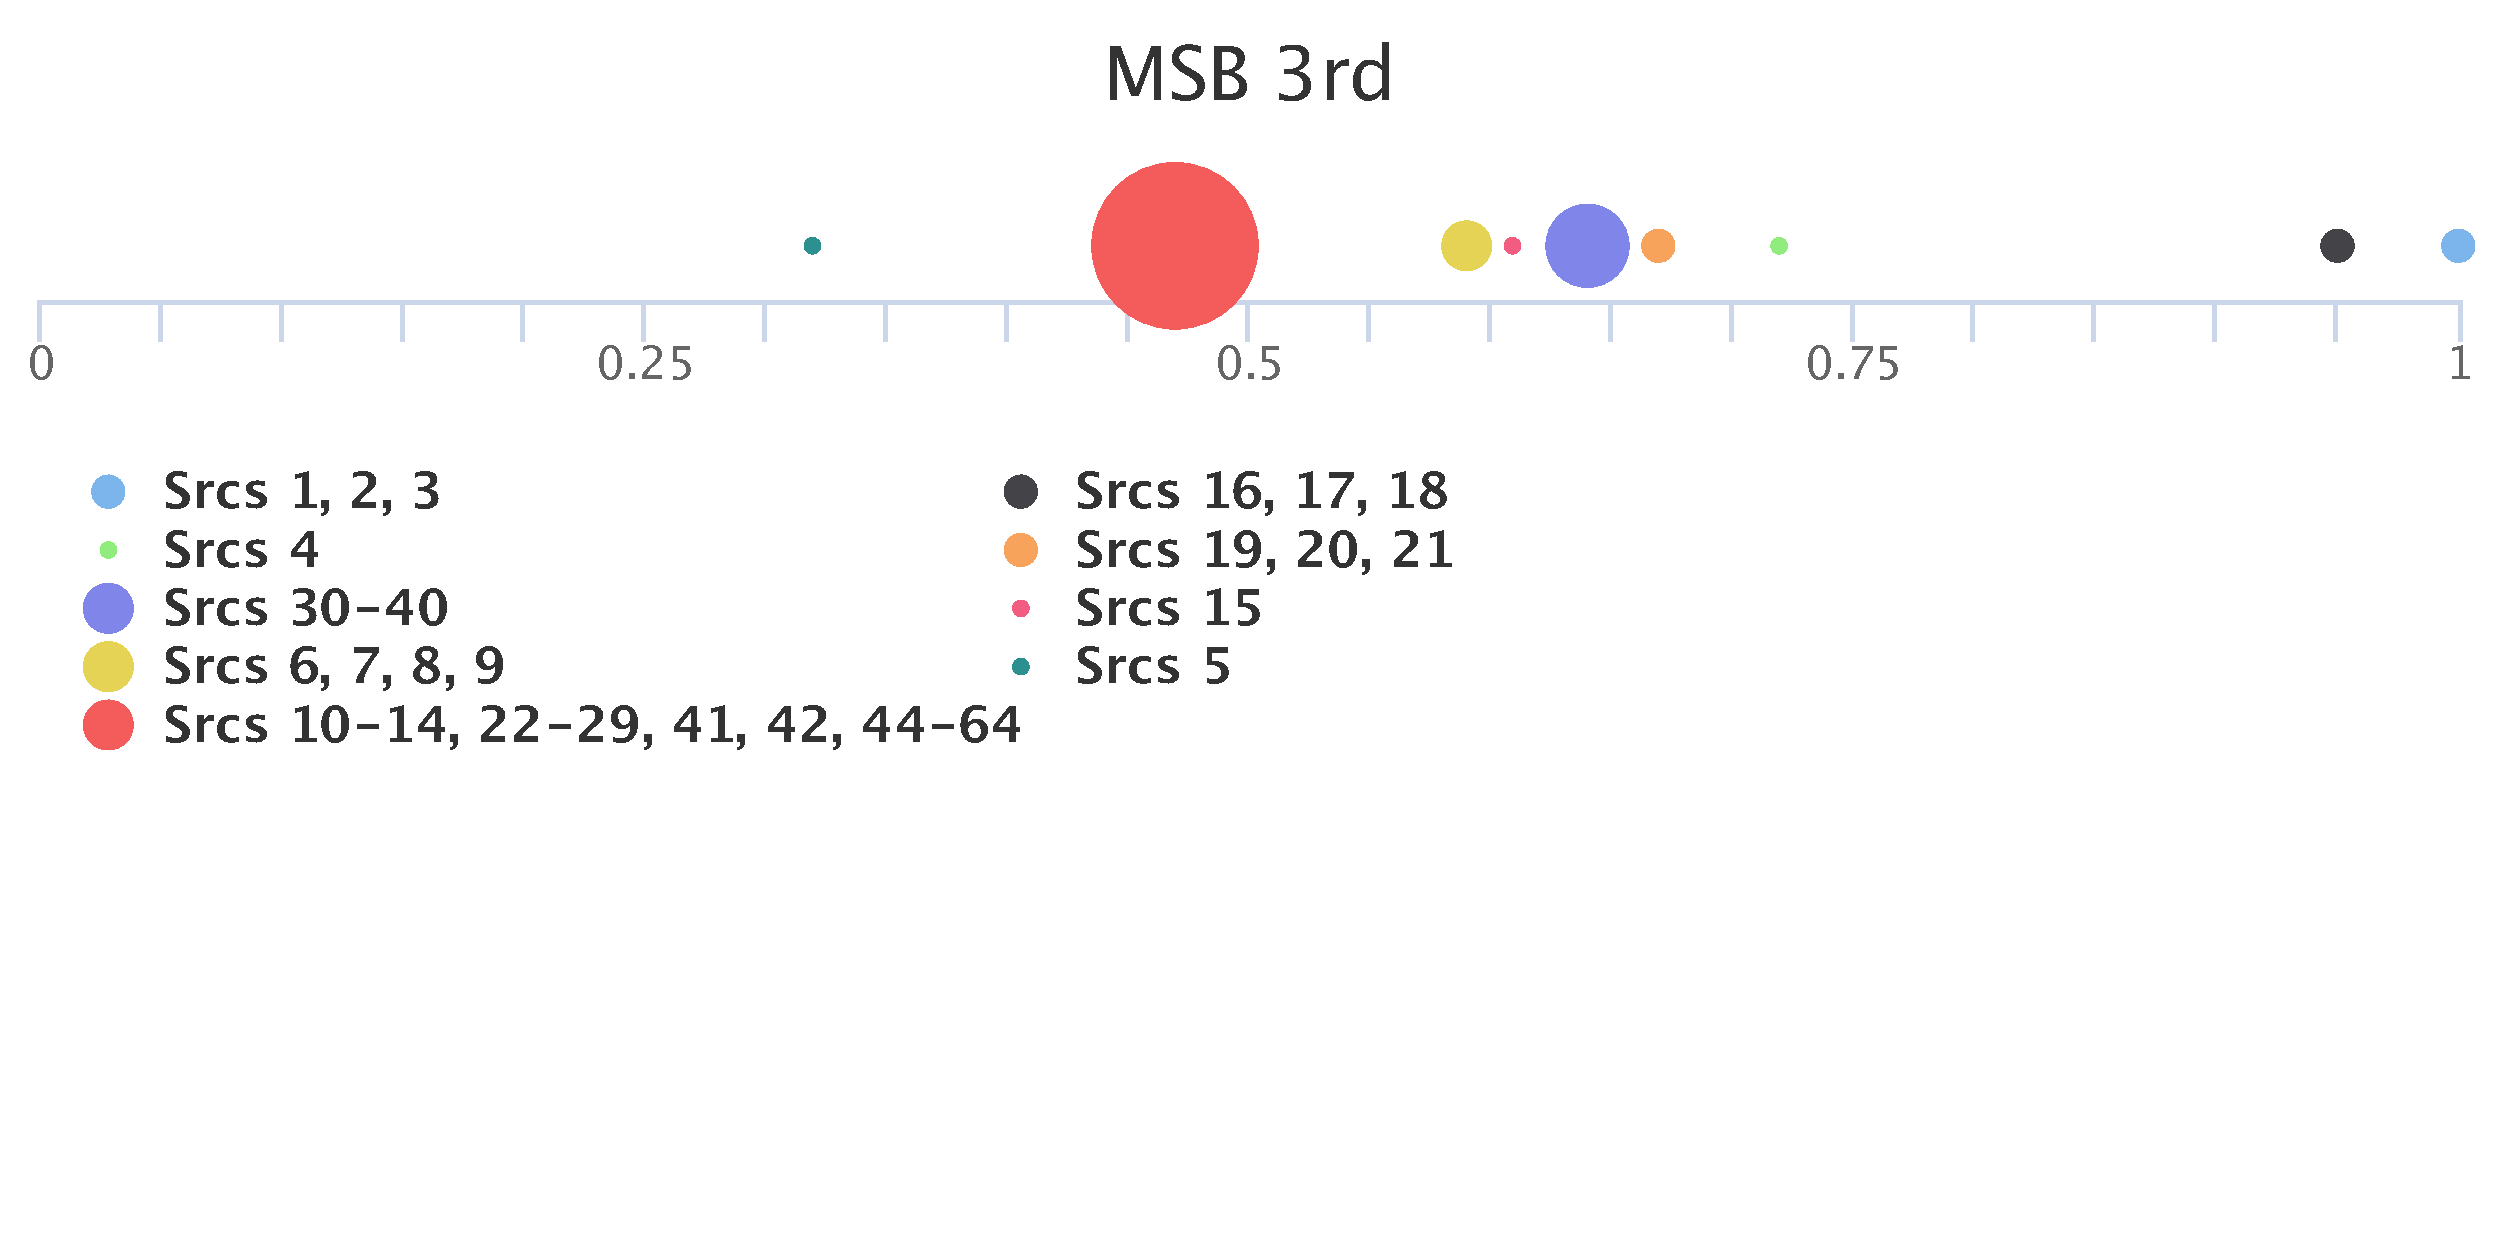
\includegraphics[width=\linewidth]{tex/images/analysis/bit3}
	\caption{Probability of 0 of 3rd most significant bit.}
\end{figure}

\begin{figure}[H]
	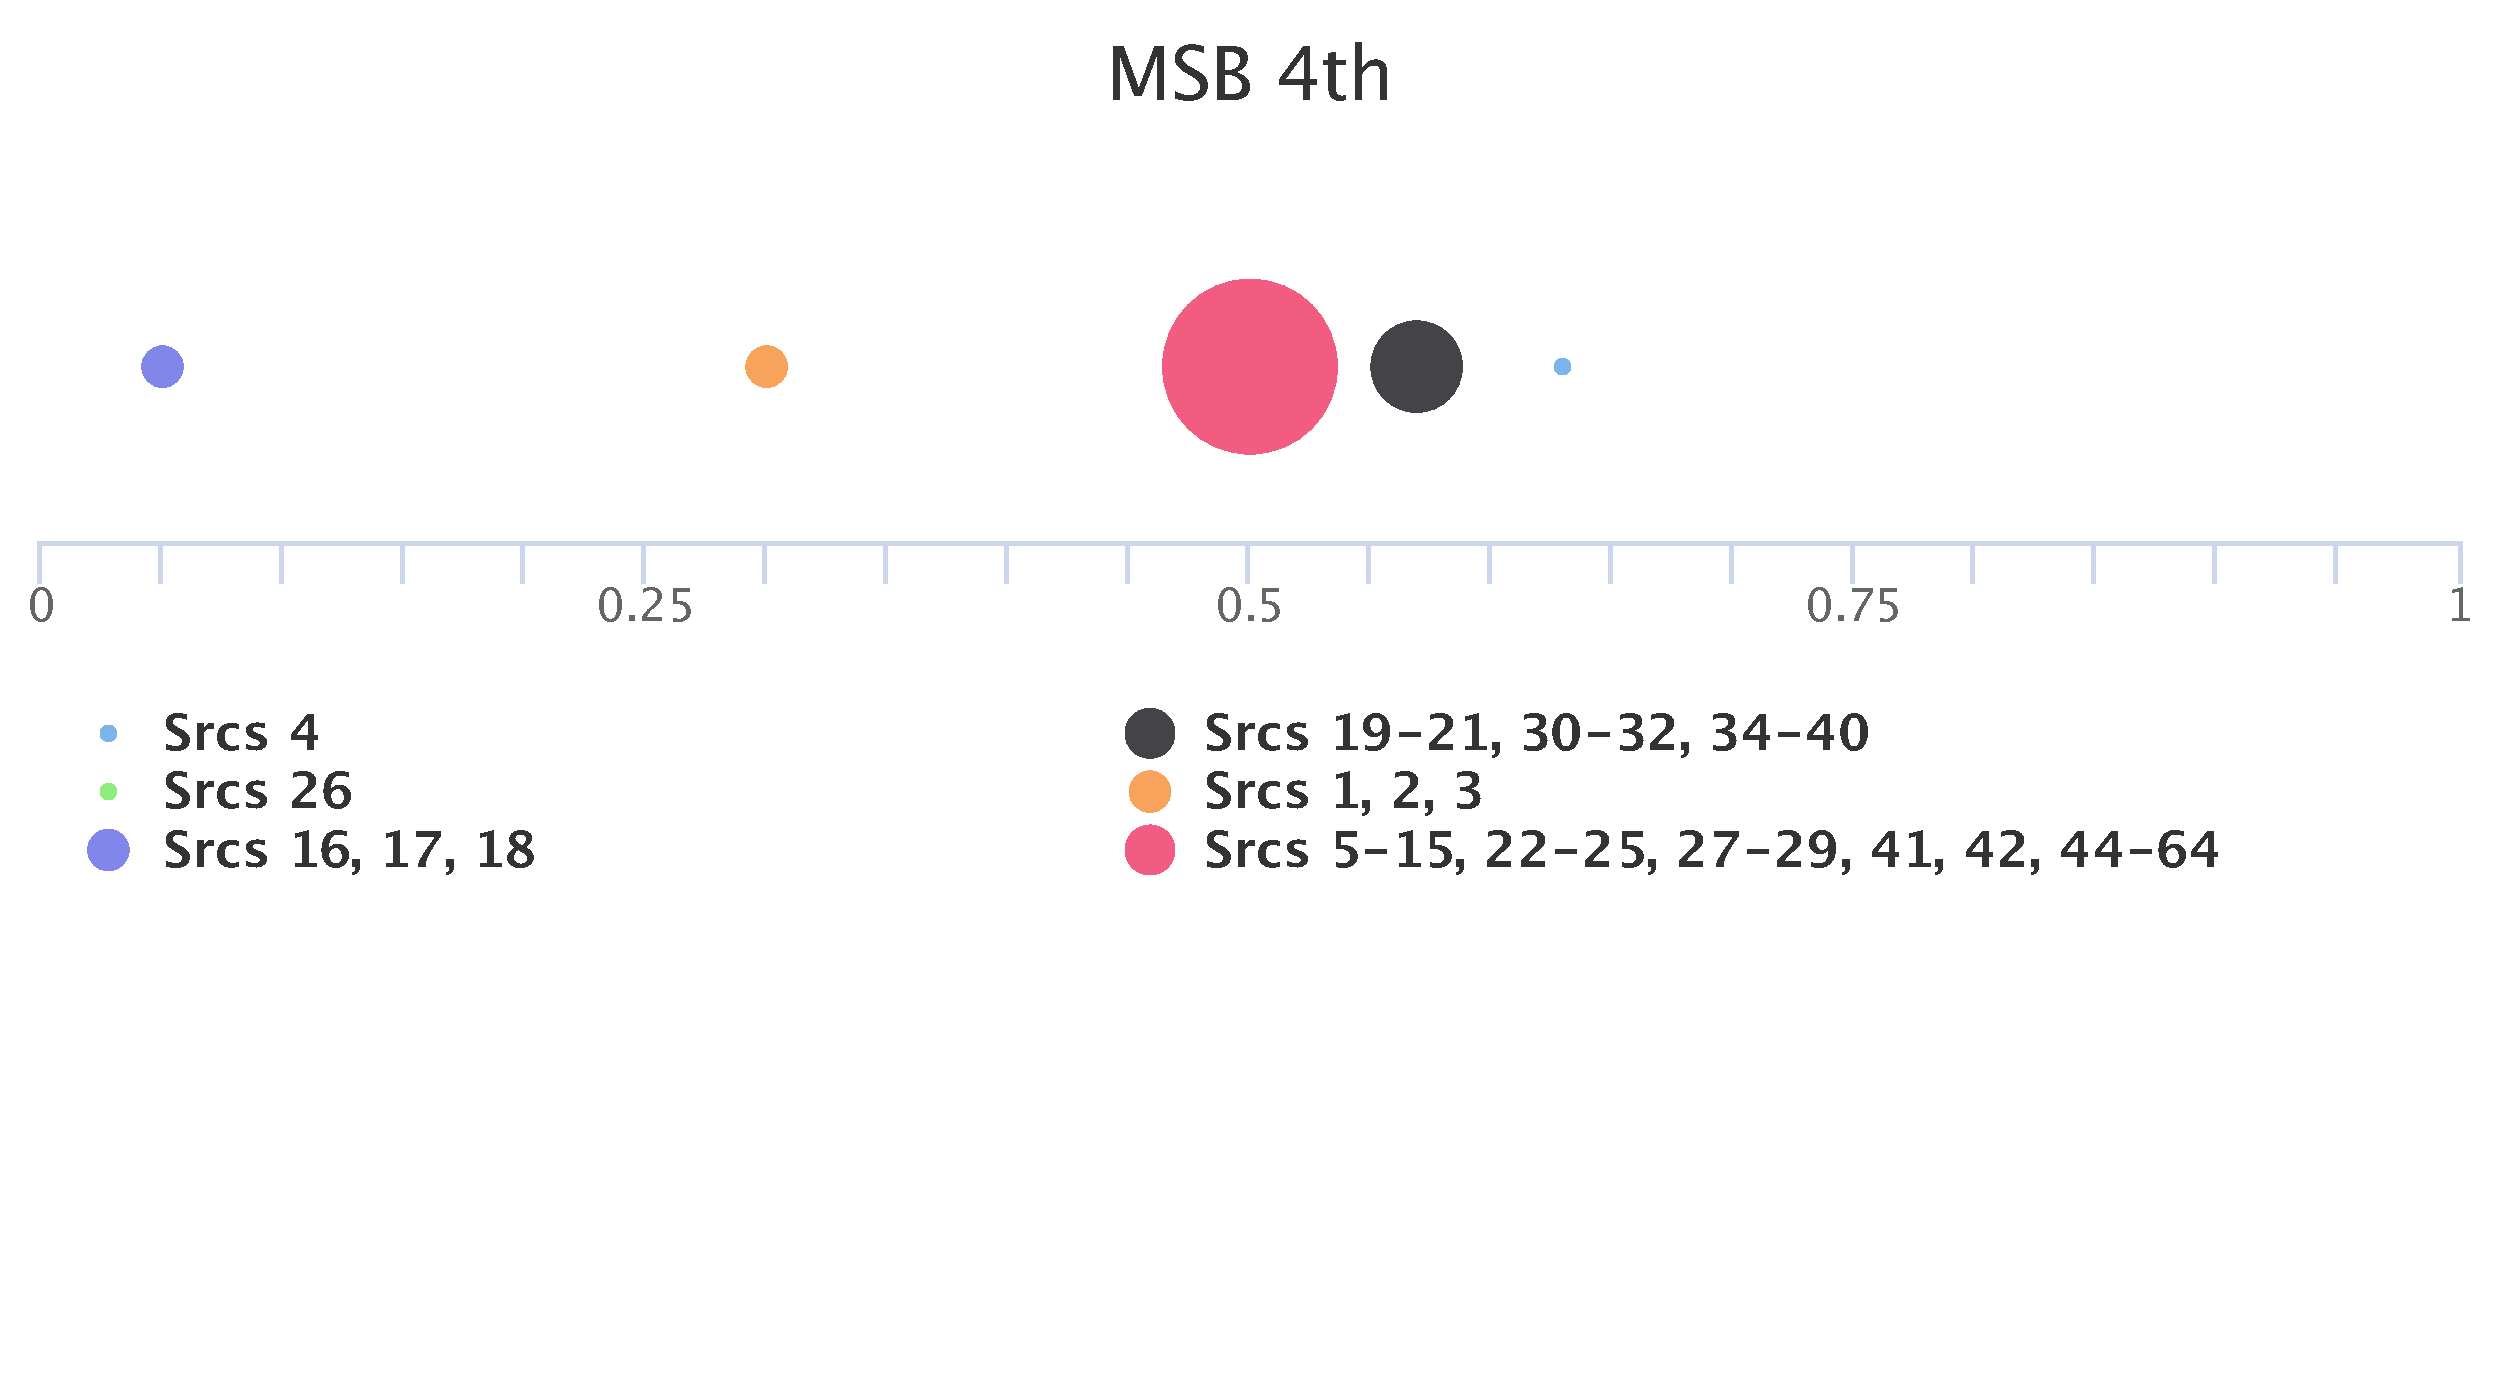
\includegraphics[width=\linewidth]{tex/images/analysis/bit4}
	\caption{Probability of 0 of 4th most significant bit.}
\end{figure}